\documentclass[11pt]{ujarticle}
%\documentclass{jlreq,11pt}
%%%%%%% スタイルファイル %%%%%%%%%%%%%%%%%%%%%%
\usepackage{lmodern}
\usepackage{amsmath,amssymb}

\usepackage{thesis}

\usepackage[dvipdfmx]{graphicx}   % pdf 形式の図版取り込みのため , draftは消す
\usepackage{ascmac}
\usepackage{multicol}
\usepackage{array}
\usepackage{float}
\usepackage{indent}
\setlength{\parindent}{1em} % 段落の字下げを2文字分にする

\usepackage{url}

\usepackage{color}
\definecolor{lightgray}{gray}{0.9}
\definecolor{darkgray}{gray}{0.25}

\usepackage{framed}
\makeatletter
\renewenvironment{leftbar}{%
  \def\FrameCommand{\hspace{1.5zw}\textcolor{darkgray}{\vrule width 2pt}\hspace{0.5zw}}% 
  \MakeFramed {\advance\hsize-\width \FrameRestore}}%
 {\endMakeFramed}
\makeatother
\usepackage{subcaption}

\usepackage{tcolorbox}
\usepackage{verbatim} % verbatim 環境を使うために必要
\tcbuselibrary{skins, listingsutf8}  % ← skins を忘れずに!

\usepackage{listings,jvlisting} 
\usepackage{xcolor} 
\usepackage{caption}
%\captionsetup[lstlisting]{labelfont=bf, font=footnotesize, format=plain, singlelinecheck=false}

\usepackage{fancyhdr}
\pagestyle{fancy}
\fancyhf{}  % 既存のヘッダー・フッターを消す
\fancyfoot[C]{\thepage}  % 中央下部にページ番号を出す
\renewcommand{\headrulewidth}{0pt}  % ヘッダー罫線を消す


\renewcommand{\lstlistingname}{Code}

\lstset{
    basicstyle=\ttfamily\scriptsize,
    keywordstyle=\color{blue},
    commentstyle=\color{gray},
    stringstyle=\color{red},
    columns=fullflexible,    % ← extendedchars の代わり
    numbers=left,
    stepnumber=1,
    numbersep=10pt,
    frame=tb,
    captionpos=b,
    breaklines=true,
    breakatwhitespace=false,
    showspaces=false,
    showstringspaces=false,
    tabsize=4,
    extendedchars=true,      
    inputencoding=utf8,       
    backgroundcolor={\color[gray]{.95}},
}




\begin{document}

%%%%%%%%%%%%%%%%%%%%%%%%%%%%%%%%%%%%%%%%%%%%%%%%%%%%%%%%%%%%%%%%%%%%%%%%%%%%%
%%%%%% 表紙 %%%%%%%%%%%%%%%%%%%%%%%%%%%%%%%%%%%%%%%%%%%%%%%%%%%%%%%%%%%%%%%
%%%%%%%%%%%%%%%%%%%%%%%%%%%%%%%%%%%%%%%%%%%%%%%%%%%%%%%%%%%%%%%%%%%%%%%%%%%%%

% === 年度を記入 ============================================================
\def\year{7}	% 令和 1 年度の場合

% === 提出年月日を記入 ============================================================
\def\submityear{7}	% 令和 7 年
\def\submitmonth{5}	% 5 月
\def\submitdate{12}	% 12 日

% === 題目を記入 ============================================================
\def\title{%
  ~2 軸ロボットの運動制御実験~   Quanser Consulting 社製 2軸ロボット
}%

% === 題目を記入(背表紙用) ============================================================
\def\spine{%
  人追従搬送ロボットのシステム開発
}%

% === 学科を記入 ==========================================================
\def\course{電気電子システム工学コース}

% === 学籍番号を記入 ========================================================
\def\student_number{a0527}

% === 氏名を記入 ============================================================
\def\name{野口 史遠}


% === 表紙 ========================================================
\thispagestyle{empty}
% !TEX root = main.tex


\newpage
% ======================================================================
\begin{center}
    {\fontsize{20pt}{0pt}\selectfont\bf{令和\ \year\ 年度}}\\[1zh]
    {\fontsize{28pt}{0pt}\selectfont\bf{\kintou{8zw}{実験レポート}}}
\end{center}
% ======================================================================
\vspace{2zh}


% ======================================================================
\begin{center}
    \fontsize{20pt}{26pt}\selectfont
    \renewcommand{\arraystretch}{1.4}
    \begin{tabular}{|p{2zw}|p{20zw}|}
        \hline
        {\bf{題目}} & 
        {\bf{\title}}  \\\hline
    \end{tabular}
\end{center}
% ======================================================================
\vspace{2zh}

% ======================================================================
\begin{center}
    \fontsize{16pt}{18pt}\selectfont
    \renewcommand{\arraystretch}{1.4}
    \tabcolsep 4pt
    \begin{tabular}{|p{4zw}|p{14zw}|}
        \hline
        {\bf{\kintou{4zw}{学科}}}     & 
        {\bf{\course}}                                                  \\\hline
        {\bf{\kintou{4zw}{学籍番号}}} & 
        {\bf{\student_number}}                                          \\\hline
        {\bf{\kintou{4zw}{氏名}}}     & 
        {\bf{\name}}                                                    \\\hline
        {\bf{\kintou{4zw}{提出日}}}   & 
        {\bf{令和\ \submityear\ 年\ \submitmonth\ 月\ \submitdate\ 日}} \\\hline
    \end{tabular}
\end{center}
% ======================================================================
\vspace{0zh}


\vfill
% ======================================================================
\begin{center}
    
\includegraphics[width=45mm]{figure/logo_maizuru_gray.pdf}
\end{center}
% ======================================================================
\vspace{0.25zh}
% ======================================================================
\begin{center}
    {\fontsize{22pt}{0pt}\selectfont\bf{舞鶴工業高等専門学校}}\\[1zh]
    {\fontsize{22pt}{0pt}\selectfont\bf{電子制御工学科}}
\end{center}
% ======================================================================


\thispagestyle{empty}
 \newpage

% === 論文要旨 ========================================================
\thispagestyle{empty}
%% !TEX root = main.tex
\begin{center}
    \section*{論\,文\,要\,旨}                      %% ここに番号をつけない
\end{center}

近年,生産年齢人口の減少が社会的な課題となっており,
ロボット技術の導入による作業の効率化が期待されている.
例えば,草刈りロボットや運搬ロボットなど,人手不足を補うための自律ロボットが徐々に普及しつつある.
しかしながら,多くの自動搬送ロボットにはLiDARや3Dセンサーなどの高価なセンサーが搭載されているケースが多い.
LiDARは高精度な距離計測を可能にし,障害物回避や人追従において重要な役割を果たす一方で,その導入コストが非常に高く,
特に中小企業や農業現場では導入が難しい現状がある.
近年,カメラ映像を用いて物体位置を認識し,自律移動を行うシステムは物流や農業,介護など幅広い分野で需要が高まっている.

本研究では,カメラのみを用いた低コストな人追従搬送ロボットの開発を目指し,
Intel RealSense D435iを使用した画像処理技術と追従制御アルゴリズムの実装に取り組んだ.

具体的には,デプスカメラから取得した深度データを用いて,画像上の座標を実空間の物理座標に変換し,人の位置を推定する.
また,追従制御には,比例航法(PN),修正比例航法(MPN),およびゲインスケジューリング下修正比例航法(GS-MPN)の3つのアルゴリズムを実装し,
それぞれの性能を比較評価した.さらに,ROS2を用いたシステム全体の統合を行い,上位層と下位層を連携させたリアルタイム制御を実現した.

実験では,ロボットが直線および曲線の軌道を持つ目標物を追従する際の精度と滑らかさを評価した.
結果として,GS-MPNが最もバランスの取れた性能を示し,急加速を抑えつつ安定した追従を実現した.
これにより,従来手法で見られた不安定な動作や追従精度の低下が大幅に改善された.
一方で,遮蔽物や複数対象物が存在する場合の課題が残されており,これらの状況に対応するための識別技術や外乱耐性の強化が今後の課題である.

本研究の成果は,コスト効率に優れた人追従ロボットの実現に向けた重要なステップとなり,
物流や医療分野など多様な応用への可能性を示唆するものである.
今後は,環境適応性の向上や予測制御技術の導入を通じて,さらに高性能で信頼性の高いロボットシステムの開発を目指す. \newpage

%%%%%%%%%%%%%%%%%%%%%%%%%%%%%%%%%%%%%%%%%%%%%%%%%%%%%%%%%%%%%%%%%%%%%%%%%%%%%
%%%%%% 目次 %%%%%%%%%%%%%%%%%%%%%%%%%%%%%%%%%%%%%%%%%%%%%%%%%%%%%%%%%%%%%%%
%%%%%%%%%%%%%%%%%%%%%%%%%%%%%%%%%%%%%%%%%%%%%%%%%%%%%%%%%%%%%%%%%%%%%%%%%%%%%
\pagenumbering{roman}
\tableofcontents         %% 目次 
\newpage

\pagenumbering{arabic}
\setcounter{page}{1}
%%%%%%%%%%%%%%%%%%%%%%%%%%%%%%%%%%%%%%%%%%%%%%%%%%%%%%%%%%%%%%%%%%%%%%%%%%%%%
%%%%%% 本文 %%%%%%%%%%%%%%%%%%%%%%%%%%%%%%%%%%%%%%%%%%%%%%%%%%%%%%%%%%%%%%%
%%%%%%%%%%%%%%%%%%%%%%%%%%%%%%%%%%%%%%%%%%%%%%%%%%%%%%%%%%%%%%%%%%%%%%%%%%%%%
% !TEX root = main.tex
\section{概要}

本実験はダイオードの特性理解からデバイス作製,評価までを行う.

第1週では,ダイオードの基本特性について学習し,実際の測定を通じてその動作原理を確認する.
具体的には,ダイオードの電流-電圧特性を測定し,以下のパラメータを抽出・解析する
\begin{itemize}
    \item 直列抵抗
    \item 並列抵抗  
    \item 理想係数n
\end{itemize}

第2週では,ダイオードの作製方法について学習し,実際にデバイスの作製を行う.この週では以下の項目の理解を目的とする.
\begin{itemize}
    \item デバイス構造の設計
    \item デバイス作製プロセスの実践
\end{itemize}

第3週では,前週で作製したダイオードデバイスの特性測定と評価を実施し,作製プロセスと得られた特性の関係について考察を行う.
 \newpage
% !TEX root = main.tex \newpage
% !TEX root = main.tex
\section{実験方法}

本実験では,段階的にWebデータベースを構築するため,複数のステップに分けて作業を行った.ここでは,まず最初に行ったXAMPPのインストールおよび動作確認について記述する.

\subsection*{環境}
\begin{itemize}
  \item OS:Ubuntu 22.04 LTS
\end{itemize}

\subsection*{実験Ⅰ:XAMPPのインストールと起動確認}

XAMPPは,Apache Webサーバ,MySQL(MariaDB),PHP,Perl などを一括でインストール・管理できるパッケージである.本実験では,XAMPPをインストールしてApacheの起動確認を行った.

\vspace{1zh}
\noindent 手順は以下の通りである.

\begin{enumerate}
  \item 以下の公式サイトより,XAMPPのLinux版インストーラをダウンロードする.
        \url{https://www.apachefriends.org/jp/index.html}

  \item ターミナルでダウンロードディレクトリに移動する.
        \begin{lstlisting}[language=bash]
cd ~/Downloads/
\end{lstlisting}

  \item インストーラに実行権限を与える.
        \begin{lstlisting}[language=bash]
sudo chmod 755 xampp-linux-x64-8.0.10-0-installer.run
\end{lstlisting}

  \item インストーラを実行する.
        \begin{lstlisting}[language=bash]
sudo ./xampp-linux-x64-8.0.10-0-installer.run
\end{lstlisting}

  \item GUIベースのマネージャを起動する.
        \begin{lstlisting}[language=bash]
sudo /opt/lampp/manager-linux-x64.run
\end{lstlisting}

  \item LAMP環境を起動する.
        \begin{lstlisting}[language=bash]
sudo /opt/lampp/lampp start
\end{lstlisting}

  \item ブラウザで \texttt{http://localhost/} を開き,「XAMPPへようこそ」と表示されればApacheの動作確認は完了である.

  \item 確認後,LAMP環境を停止する.
        \begin{lstlisting}[language=bash]
sudo /opt/lampp/lampp stop
\end{lstlisting}


\end{enumerate}

この操作により,Webサーバの動作環境が整い,今後のWebデータベース構築に必要な基盤が準備された.

\begin{figure}[htbp]
  \centering
  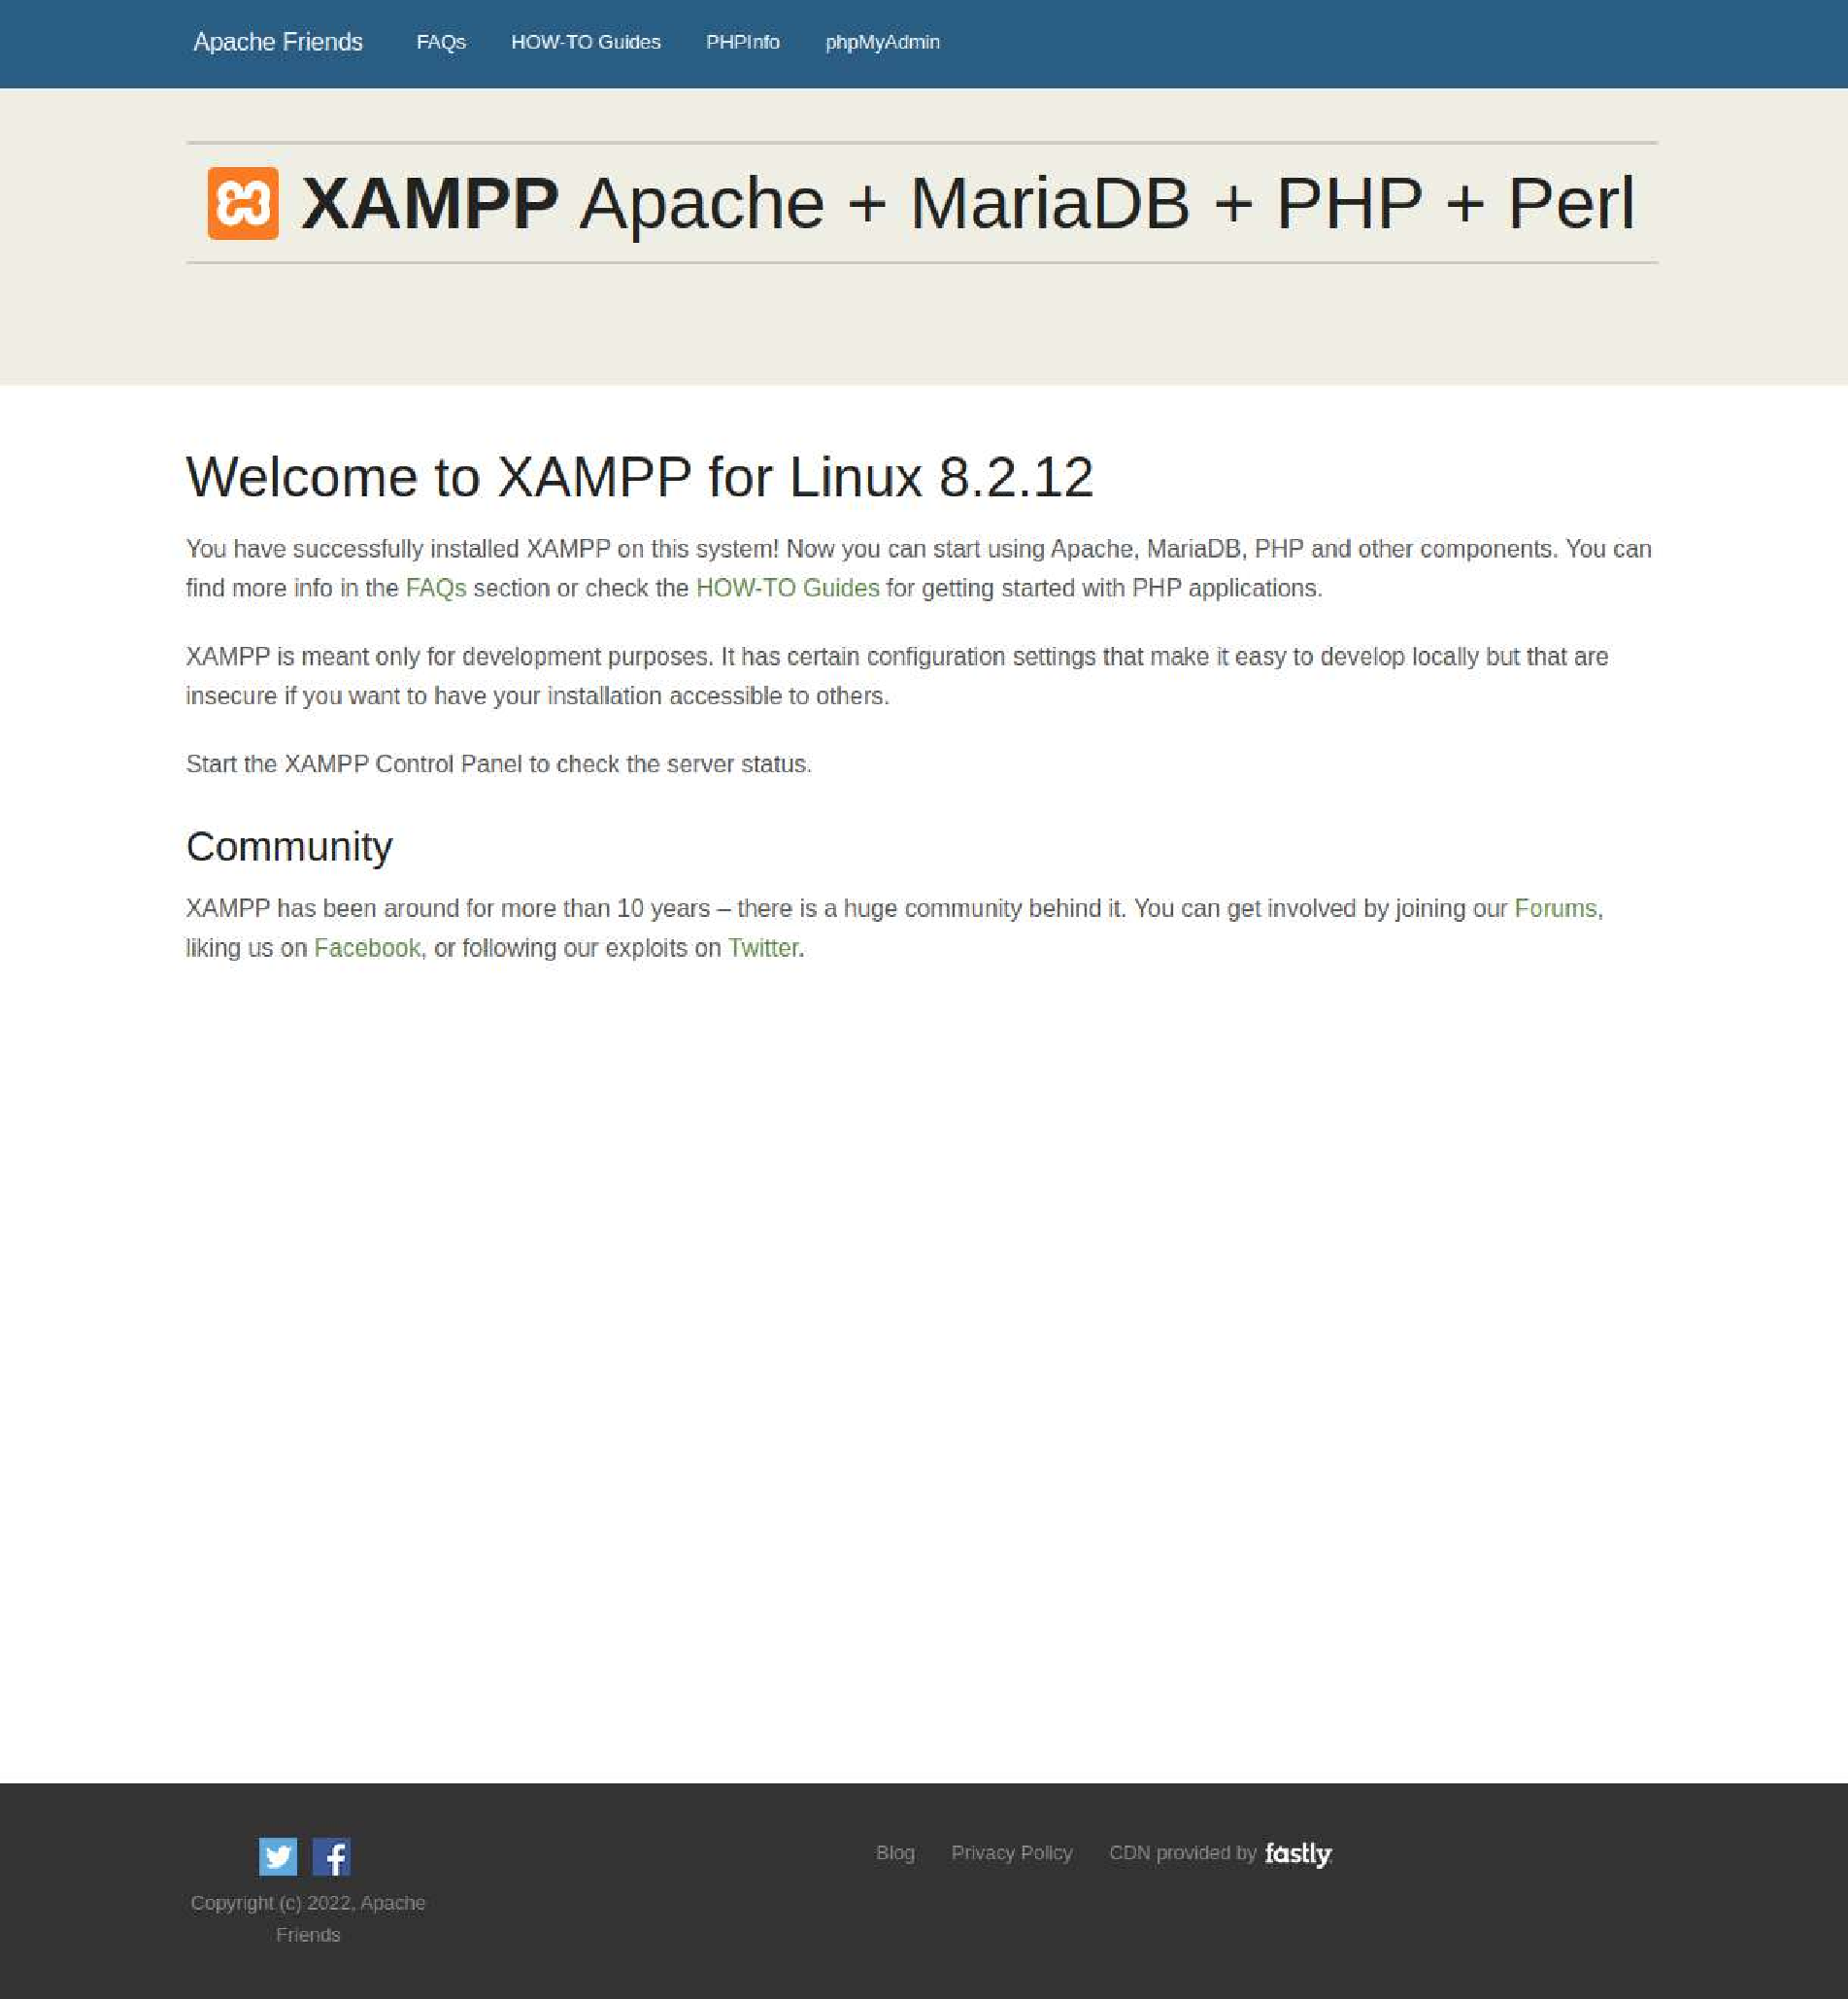
\includegraphics[width=0.9\linewidth]{figure/1.pdf}
  \caption{Welcome to XAMPP}
\end{figure}

\subsection*{実験Ⅱ:Webページ作成とデータベース構築}

本実験では,HTMLによるWebページの作成と,phpMyAdminを用いたデータベース(MariaDB)の作成・検索,およびPHPを用いたWebデータベースの構築を行った.

\subsubsection*{1. Webページの作成}

XAMPPのドキュメントルートに移動し,HTMLファイルを作成した.

\begin{lstlisting}[language=bash]
cd /opt/lampp/htdocs/
\end{lstlisting}

作成したファイル \texttt{sample.html} は以下の通りである.

\begin{lstlisting}[language=html]
<!DOCTYPE html>
<html>
<head>
<meta http-equiv="Content-Type" content="text/html; charset=utf-8"/>
<title>こんにちは</title>
</head>
<body>
<h1>見出し</h1>
<p>文章を書きましょう</p>
</body>
</html>
\end{lstlisting}

これをブラウザで \texttt{http://localhost/sample.html} にアクセスすることで表示を確認した.

次に,CSSによって文字色を赤く変更したスタイルを追加した.

\begin{lstlisting}[language=html]
<style>
 p {
   color: red;
 }
</style>
\end{lstlisting}

\begin{figure}[htbp]
  \centering
  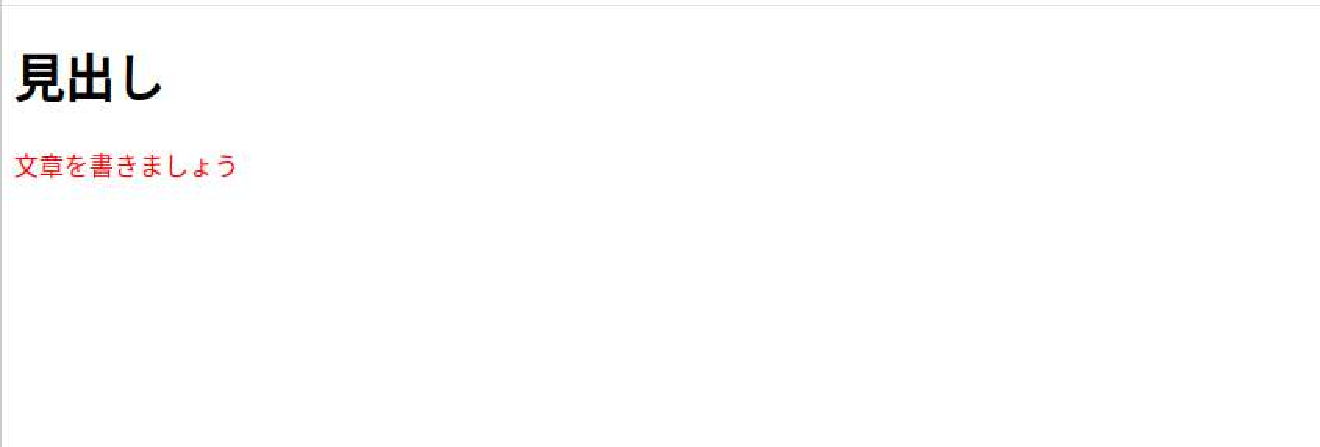
\includegraphics[width=0.9\linewidth]{figure/2.pdf}
  \caption{sample.html}
\end{figure}

\subsubsection*{2. データベースの作成・検索}

\texttt{phpMyAdmin}を用いて,データベース \texttt{maizuru} を作成し,以下の2つのテーブルを構築した.

\vspace{0.5zh}
\begin{itemize}
  \item \textbf{nameテーブル}:no, name(TEXT型)
  \item \textbf{birthplaceテーブル}:name, birthplace(TEXT型)
\end{itemize}

データを追加後,以下のSQL文でデータを検索・表示した.

\begin{lstlisting}[language=SQL]
SELECT * FROM name;
\end{lstlisting}

\begin{figure}[htbp]
  \centering
  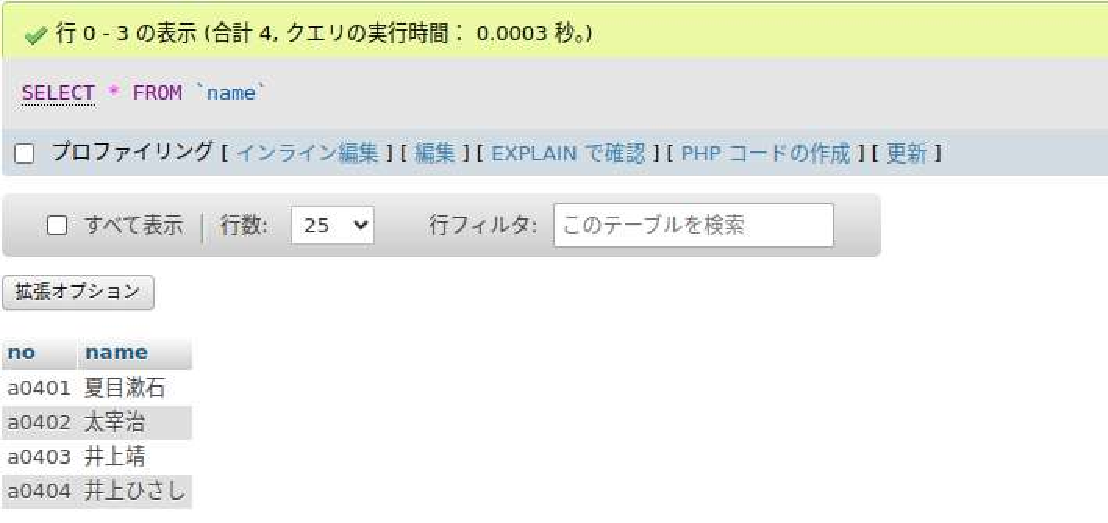
\includegraphics[width=0.9\linewidth]{figure/3.pdf}
  \caption{\texttt{maizuru} のnameテーブル}
\end{figure}

\begin{figure}[htbp]
  \centering
  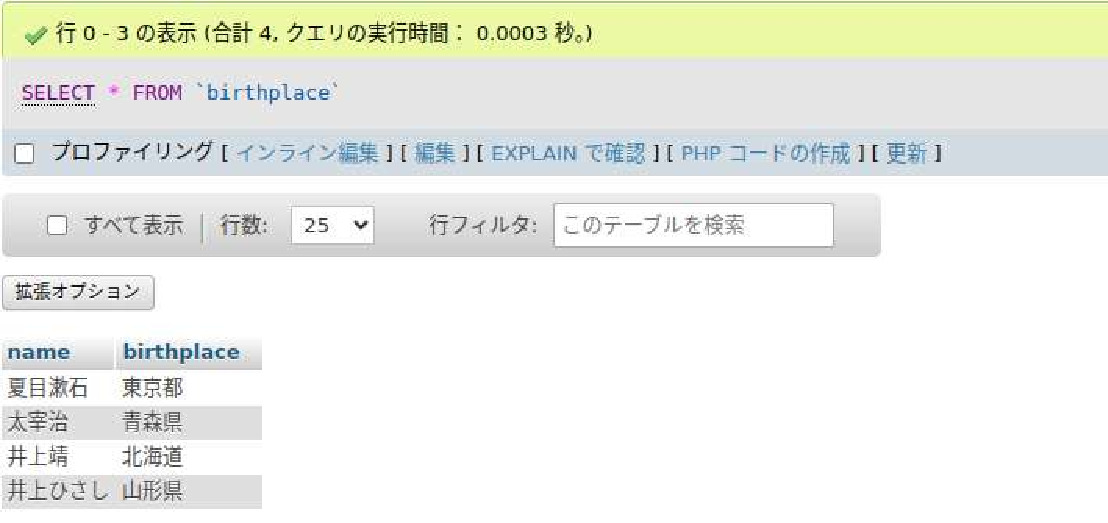
\includegraphics[width=0.9\linewidth]{figure/4.pdf}
  \caption{\texttt{maizuru} のbirthplaceテーブル}
\end{figure}

さらに,2つのテーブルを結合して,対応する生誕地を表示するクエリを実行した.

\begin{lstlisting}[language=SQL]
SELECT name.no, name.name, birthplace.birthplace 
FROM name 
INNER JOIN birthplace 
ON name.name = birthplace.name;
\end{lstlisting}

\subsubsection*{3. Webデータベースの構築(PHP)}

MariaDBのパスワードを設定するため,\texttt{--skip-grant-tables} モードで起動し,次のコマンドでパスワードを直接設定した.

\begin{lstlisting}[language=bash]
sudo /opt/lampp/sbin/mysqld --skip-grant-tables --skip-networking &
sudo /opt/lampp/bin/mysql -u root

UPDATE mysql.user 
SET authentication_string = PASSWORD('password') 
WHERE User = 'root' AND Host = 'localhost';
FLUSH PRIVILEGES;
sudo killall mysqld
sudo /opt/lampp/lampp start
\end{lstlisting}

その後,PHPを用いた接続確認とデータ表示のため,以下のファイルを配置した.

\textbf{connect.php}
\begin{lstlisting}[language=php]
    <html>
    <head>
    <meta http-equiv="Content-Type" content="text/html; charset=utf-8"/>
    <title>PHP TEST</title>
    </head>
    <body>
    
    <?php
    
    $link = mysqli_connect('localhost', 'root', 'password');
    if (!$link) {
        die('接続失敗です。'.mysql_error());
    }
    
    print('<p>接続に成功しました。</p>');
    
    $db_selected = mysqli_select_db($link,'maizuru');
    if (!$db_selected){
        die('データベース選択失敗です。'.mysql_error());
    }
    
    print('<p>データベースを選択しました。</p>');
    
    // MySQLに対する処理
    
    $close_flag = mysqli_close($link);
    
    if ($close_flag){
        print('<p>切断に成功しました。</p>');
    }
    
    ?>
    </body>
    </html>
\end{lstlisting}

\begin{figure}[htbp]
  \centering
  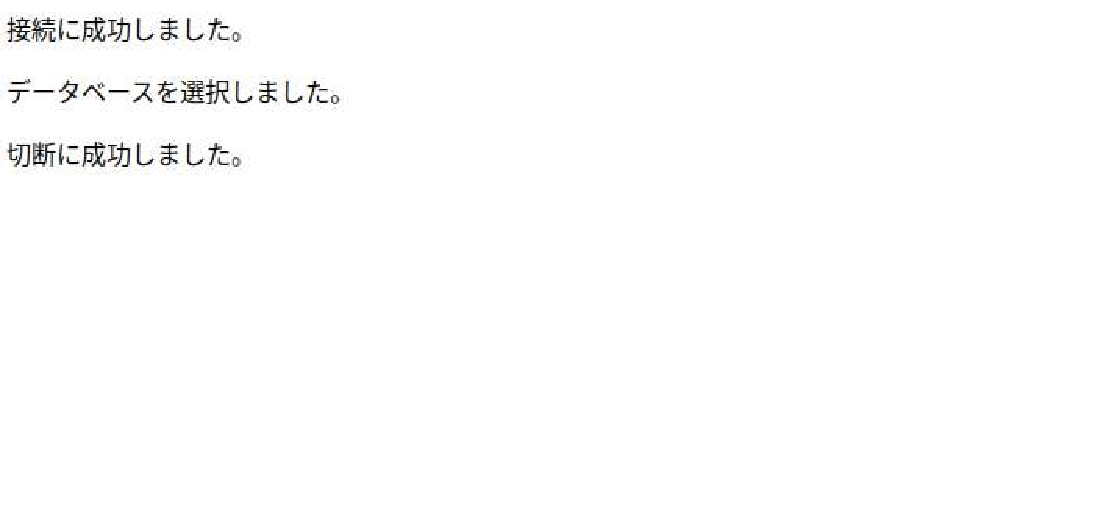
\includegraphics[width=0.9\linewidth]{figure/6.pdf}
  \caption{connect.php}
\end{figure}

\textbf{select.php}
\begin{lstlisting}[language=php]
    <html>
    <head>
    <meta http-equiv="Content-Type" content="text/html; charset=utf-8"/>
    <title>PHP TEST</title>
    </head>
    <body>
    
    <?php
    
    $link = mysqli_connect('localhost', 'root', 'password');
    if (!$link) {
        die('接続失敗です。'.mysql_error());
    }
    
    print('<p>接続に成功しました。</p>');
    
    $db_selected = mysqli_select_db($link,'maizuru');
    if (!$db_selected){
        die('データベース選択失敗です。'.mysqli_error());
    }
    
    print('<p>データベースを選択しました。</p>');
    
    mysqli_set_charset($link,'utf8');
    
    $result = mysqli_query($link,'SELECT * FROM name');
    if (!$result) {
        die('クエリーが失敗しました。'.mysql_error());
    }
    
    while ($row = mysqli_fetch_assoc($result)) {
        print('<p>');
        print('id='.$row['no']);
        print(', name='.$row['name']);
        print('</p>');
    }
    
    $close_flag = mysqli_close($link);
    
    if ($close_flag){
        print('<p>切断に成功しました。</p>');
    }
    
    ?>
    </body>
    </html>
\end{lstlisting}
\begin{figure}[htbp]
  \centering
  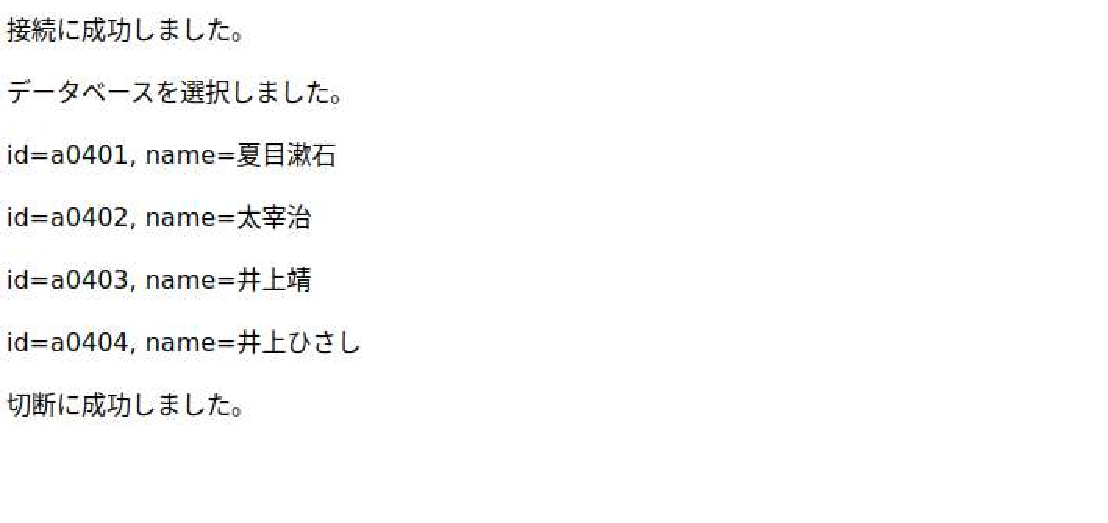
\includegraphics[width=0.9\linewidth]{figure/7.pdf}
  \caption{select.php}
\end{figure}

\textbf{select2.php}
\begin{lstlisting}[language=php]
    <html>
    <head>
    <meta http-equiv="Content-Type" content="text/html; charset=utf-8"/>
    <title>PHP TEST</title>
    </head>
    <body>
    
    <?php
    
    $link = mysqli_connect('localhost', 'root', 'password');
    if (!$link) {
        die('接続失敗です。'.mysql_error());
    }
    
    print('<p>接続に成功しました。</p>');
    
    $db_selected = mysqli_select_db($link,'maizuru');
    if (!$db_selected){
        die('データベース選択失敗です。'.mysql_error());
    }
    
    print('<p>データベースを選択しました。</p>');
    
    mysqli_set_charset($link,'utf8');
    
    $result = mysqli_query($link,'SELECT name.no, name.name, birthplace.birthplace FROM name inner join birthplace on name.name=birthplace.name');
    if (!$result) {
        die('クエリーが失敗しました。'.mysqli_error());
    }
    
    while ($row = mysqli_fetch_assoc($result)) {
        print('<p>');
        print('id='.$row['no']);
        print(', name='.$row['name']);
        print(', birthplace='.$row['birthplace']);
        print('</p>');
    }
    
    $close_flag = mysqli_close($link);
    
    if ($close_flag){
        print('<p>切断に成功しました。</p>');
    }
    
    ?>
    </body>
    </html>
\end{lstlisting}
\begin{figure}[htbp]
  \centering
  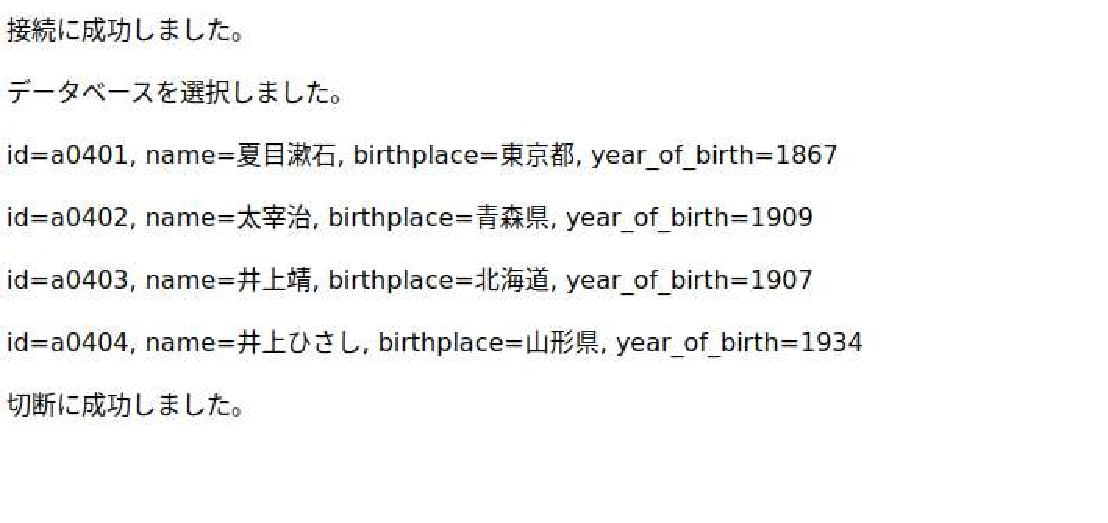
\includegraphics[width=0.9\linewidth]{figure/8.pdf}
  \caption{select2.php}
\end{figure}

\textbf{form\_name.html}(入力フォーム)

\begin{lstlisting}[language=html]
  <html>

  <head>
    <meta http-equiv="Content-Type" content="text/html; charset=utf-8" />
    <title>検索</title>
  </head>
  
  <body>
    <form action="regist.php" method="post">
      番号:<br />
      <input type="text" name="no" size="30" value="" /><br />
      名前:<br />
      <input type="text" name="name" size="30" value="" /><br />
      出身地:<br />
      <input type="text" name="birthplace" size="30" value="" /><br />
      生年:<br />
      <input type="text" name="year_of_birth" size="30" value="" /><br />
      <br />
      <input type="submit" value="登録する" />
    </form>
  </body>
  
  </html>
\end{lstlisting}
\begin{figure}[htbp]
  \centering
  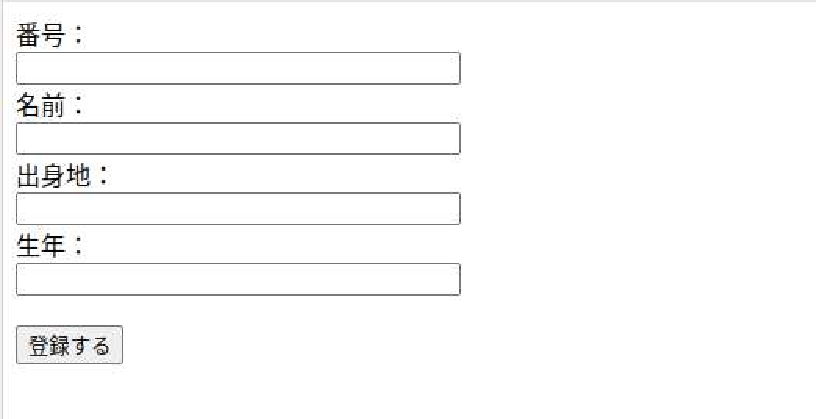
\includegraphics[width=0.9\linewidth]{figure/9.pdf}
  \caption{form\_name.html}
\end{figure}


これにより,Webフォームからデータベースへ動的に登録し,登録結果を確認する一連のWebデータベース操作が可能となった.

\subsection*{実験Ⅲ:Google Maps API を活用した Web データベースの構築}

本実験では,Google Maps API を活用して,データベースに登録された地理情報を地図上に可視化する Web アプリケーションを構築した.

\subsubsection*{1. データベースの作成}

phpMyAdmin にて,データベース \texttt{map} を新規作成し,以下の構成で \texttt{markers} テーブルを作成した.

\begin{lstlisting}[language=SQL]
CREATE TABLE `markers` ( 
  `id` INT NOT NULL AUTO_INCREMENT PRIMARY KEY, 
  `name` VARCHAR(60) NOT NULL, 
  `address` VARCHAR(80) NOT NULL, 
  `lat` FLOAT(10,6) NOT NULL, 
  `lng` FLOAT(10,6) NOT NULL, 
  `type` VARCHAR(30) NOT NULL 
) ENGINE = MYISAM;
\end{lstlisting}

初期データとして以下のようなレコードを登録した.

\begin{lstlisting}[language=SQL]
INSERT INTO `markers` (`name`, `address`, `lat`, `lng`, `type`)
VALUES ('Love.Fish', '580 Darling Street, Rozelle, NSW', -33.861034, 151.171936, 'restaurant');
\end{lstlisting}

\subsubsection*{2. データ出力用PHPスクリプト}

登録されたデータを XML 形式で出力するため,\texttt{toxml.php} を作成した.このスクリプトは,SQL クエリにより \texttt{markers} テーブルから全レコードを取得し,Google Maps JavaScript API が読み取れる形式の XML に変換して出力する.

\subsubsection*{3. Google Maps APIによる表示ページの構築}

\texttt{gis01.html},\texttt{gis02.html},\texttt{index.html} を作成し,Google Maps 上にマーカーとしてデータを描画した.

\paragraph*{gis01.html}
基本的な地図表示を行うページであり,以下のように初期表示位置とズームレベルを設定している:

\begin{lstlisting}[language=javascript]
map = new google.maps.Map(document.getElementById('map'), {
  center: {lat: -34.397, lng: 150.644},
  zoom: 8
});
\end{lstlisting}

\paragraph*{gis02.html}
\texttt{toxml.php} から取得した XML を解析し,地図上に各マーカーを配置する.

\paragraph*{index.html}
ユーザが地図上で検索できる UI を提供する.JavaScript(\texttt{script.js})により,検索ボックスやマーカーの追加が行われ,より直感的な操作が可能となる.

\subsubsection*{4. JavaScript によるマーカー描画(script.js)}

Google Maps API の \texttt{places} ライブラリと非同期通信(AJAX)を利用し,XML データを解析して地図上にマーカーを配置する処理は以下の通りである.

\begin{lstlisting}[language=javascript]
downloadUrl('toxml.php', function(data) {
  var xml = data.responseXML;
  var markers = xml.documentElement.getElementsByTagName('marker');
  ...
  var marker = new google.maps.Marker({
    map: map,
    position: point,
    label: icon.label
  });
\end{lstlisting}

マーカーをクリックすると,施設名と住所を表示する情報ウィンドウが開くように設定している.

 \newpage
\section{時間応答に基づくパラメータ同定}
\subsection{パラメータ同定とは?}

制御対象の物理パラメータの値は,はかりやメジャーなどの測定器で直接はかることができるとは限らない.
制御対象の物理パラメータの値がわからないと,制御対象の数学モデルに基づいたコントローラ設計やシミュレーションを行うことができない.
そこで,測定器で直接はかることができない物理パラメータを定めるため,制御対象に様々な信号を加え,このときの出力応答から物理パラメータの値を定める必要がある.このことを\textbf{パラメータ同定}と呼ぶ.

本実験装置の場合,\ref{sec:2_1} 節で述べたように,$v_x(t)$,$v_y(t)$ から $\theta_x(t)$,$\theta_y(t)$ への伝達関数 $G_x(s)$,$G_y(s)$ は
\begin{equation}
\left\{
\begin{aligned}
G_x(s) &= \frac{b_x}{s(s + a_x)}, \quad a_x = \frac{c_x}{J_x}, \quad b_x = \frac{k_{fx}}{J_x}, \\
G_y(s) &= \frac{b_y}{s(s + a_y)}, \quad a_y = \frac{c_y}{J_y}, \quad b_y = \frac{k_{fy}}{J_y}
\end{aligned}
\right.
\label{eq:gx_gy_transfer}
\end{equation}

であるから,$a_x$,$b_x$,$a_y$,$b_y$ の値を実験により定めることになる.
パラメータ同定を行う方法には,ステップ応答などの時間応答に基づく方法と周波数応答に基づく方法があるが,ここでは,時間応答に基づく方法を用いる.

\subsection{パラメータ同定の手順}

\paragraph{Pコントローラ}

\begin{equation}
    v_x(t) = k_{Px}(\theta_x^{\mathrm{ref}}(t) - \theta_x(t)) \tag{4.2}
\end{equation}

によりリンク1の関節角 $\theta_x(t)$ を制御したとき,2軸ロボットの数学モデル(式(2.4))と仮定すると,$\theta_x^{\mathrm{ref}}(s)$ から $\theta_x(s)$ への伝達関数は2次遅れ系

\begin{align}
    T_x(s) = \frac{G_x(s)k_{Px}}{1 + G_x(s)k_{Px}} = \frac{b_x k_{Px}}{s^2 + a_x s + b_x k_{Px}} = \frac{\omega_{nx}^2}{s^2 + 2 \zeta_x \omega_{nx} s + \omega_{nx}^2} \tag{4.3}
\end{align}

\[
\left\{
\begin{aligned}
    &\text{固有角周波数:} && \omega_{nx} = \sqrt{b_x k_{Px}} \\
    &\text{減衰係数:} && \zeta_x = \frac{a_x}{2 \omega_{nx}} = \frac{a_x}{2\sqrt{b_x k_{Px}}}
\end{aligned}
\right. \tag{4.4}
\]

となる.

(4.4)式から明らかなように,比例ゲイン $k_{Px}$ を大きくすると $\zeta_x$ は零に近づくため,ステップ応答はオーバーシュートが生じ,振動的になっていく.そこで,ある程度大きな比例ゲイン $k_{Px}$ を設定し,
目標値を

\begin{equation}
    \theta_x^{\mathrm{ref}}(t) = 
    \begin{cases}
        0 & (t < 0) \\
        \theta_{dx} & (t \geq 0)
    \end{cases} \tag{4.5}
\end{equation}

としたステップ応答にオーバシュートを生じさせると,最大ピーク値 $\max \theta_x$ と行き過ぎ時間 $t_{px}$ は以下のようになる.

\begin{equation}
    \left\{
    \begin{aligned}
        \max \theta_x &= \theta_{dx} \left(1 + \exp\left(-\frac{\gamma_x \pi}{\delta_x} \right) \right) \\
        t_{px} &= \frac{\pi}{\delta_x}
    \end{aligned}
    \right. \tag{4.6}
\end{equation}


ただし,

\begin{equation}
    \delta_x = \zeta_x \omega_{nx}, \quad \gamma_x = \omega_{nx} \sqrt{1 - \zeta_x^2} \tag{4.7}
\end{equation}

以上のことから,未知パラメータ $a_x$,$b_x$ の同定手順は以下のようになる.

パラメータ同定の手順
    \begin{enumerate}
        \item ある程度大きい比例ゲイン $k_{Px}$ を設定し,Pコントローラによるリンク1の角度制御を行う.ただし,$\theta_{dx}$ はあまり大きく設定しないようにする.たとえば,$k_{Px} = 20$,$\theta_{dx} = 0.2$ とする.
    
        \item 1) で設定した $k_{Px}$,$\theta_{dx}$ を用いて実機実験を行い,$\theta_x(t)$ をデータ列 $\theta_x^{\mathrm{data}}$ として取得する.
    
        \item 2) で取得したデータ $\theta_x^{\mathrm{data}}$ の最大値 $\max \theta_x^{\mathrm{data}}$ とそのときの時間 $t_{px}^{\mathrm{data}}$ を求める.
    
        \item $\gamma_x$,$\delta_x$ の同定値を以下の式により導出する:
        \[
            \gamma_x^{\mathrm{data}} = -\frac{1}{t_{px}^{\mathrm{data}}} \log_e \left( \frac{\max \theta_x^{\mathrm{data}}}{\theta_{dx}} - 1 \right) \tag{4.8}
        \]
        \[
            \delta_x^{\mathrm{data}} = \frac{\pi}{t_{px}^{\mathrm{data}}} \tag{4.9}
        \]
    
        \item 固有角周波数 $\omega_{nx}$,減衰係数 $\zeta_x$ の同定値を以下で定める:
        \[
            \omega_{nx}^{\mathrm{data}} = \sqrt{ (\gamma_x^{\mathrm{data}})^2 + (\delta_x^{\mathrm{data}})^2 } \tag{4.10}
        \]
        \[
            \zeta_x^{\mathrm{data}} = \frac{\gamma_x^{\mathrm{data}}}{\omega_{nx}^{\mathrm{data}}} \tag{4.11}
        \]
    
        \item $a_x$,$b_x$ の同定値 $a_x^{\mathrm{data}}$,$b_x^{\mathrm{data}}$ を次式により定める:
        \[
            a_x^{\mathrm{data}} = 2 \zeta_x^{\mathrm{data}} \omega_{nx}^{\mathrm{data}} \tag{4.12}
        \]
        \[
            b_x^{\mathrm{data}} = \frac{(\omega_{nx}^{\mathrm{data}})^2}{k_{Px}} \tag{4.13}
        \]
    \end{enumerate}
    
なお,未知パラメータ $a_y$,$b_y$ の同定手順は $a_x$,$b_x$ の同定手順と同様なので,ここでは省略する.

\noindent
\textbf{ステップ 1}:
まず,MATLAB/Simulink を起動し,以下の M ファイル ``\texttt{idarm.m}'' と
実機実験モデル ``\texttt{ex\_P.slx}'' を作成し,フォルダ \texttt{\textyen ID} に保存する.

\begin{figure}[htbp]
    \centering
    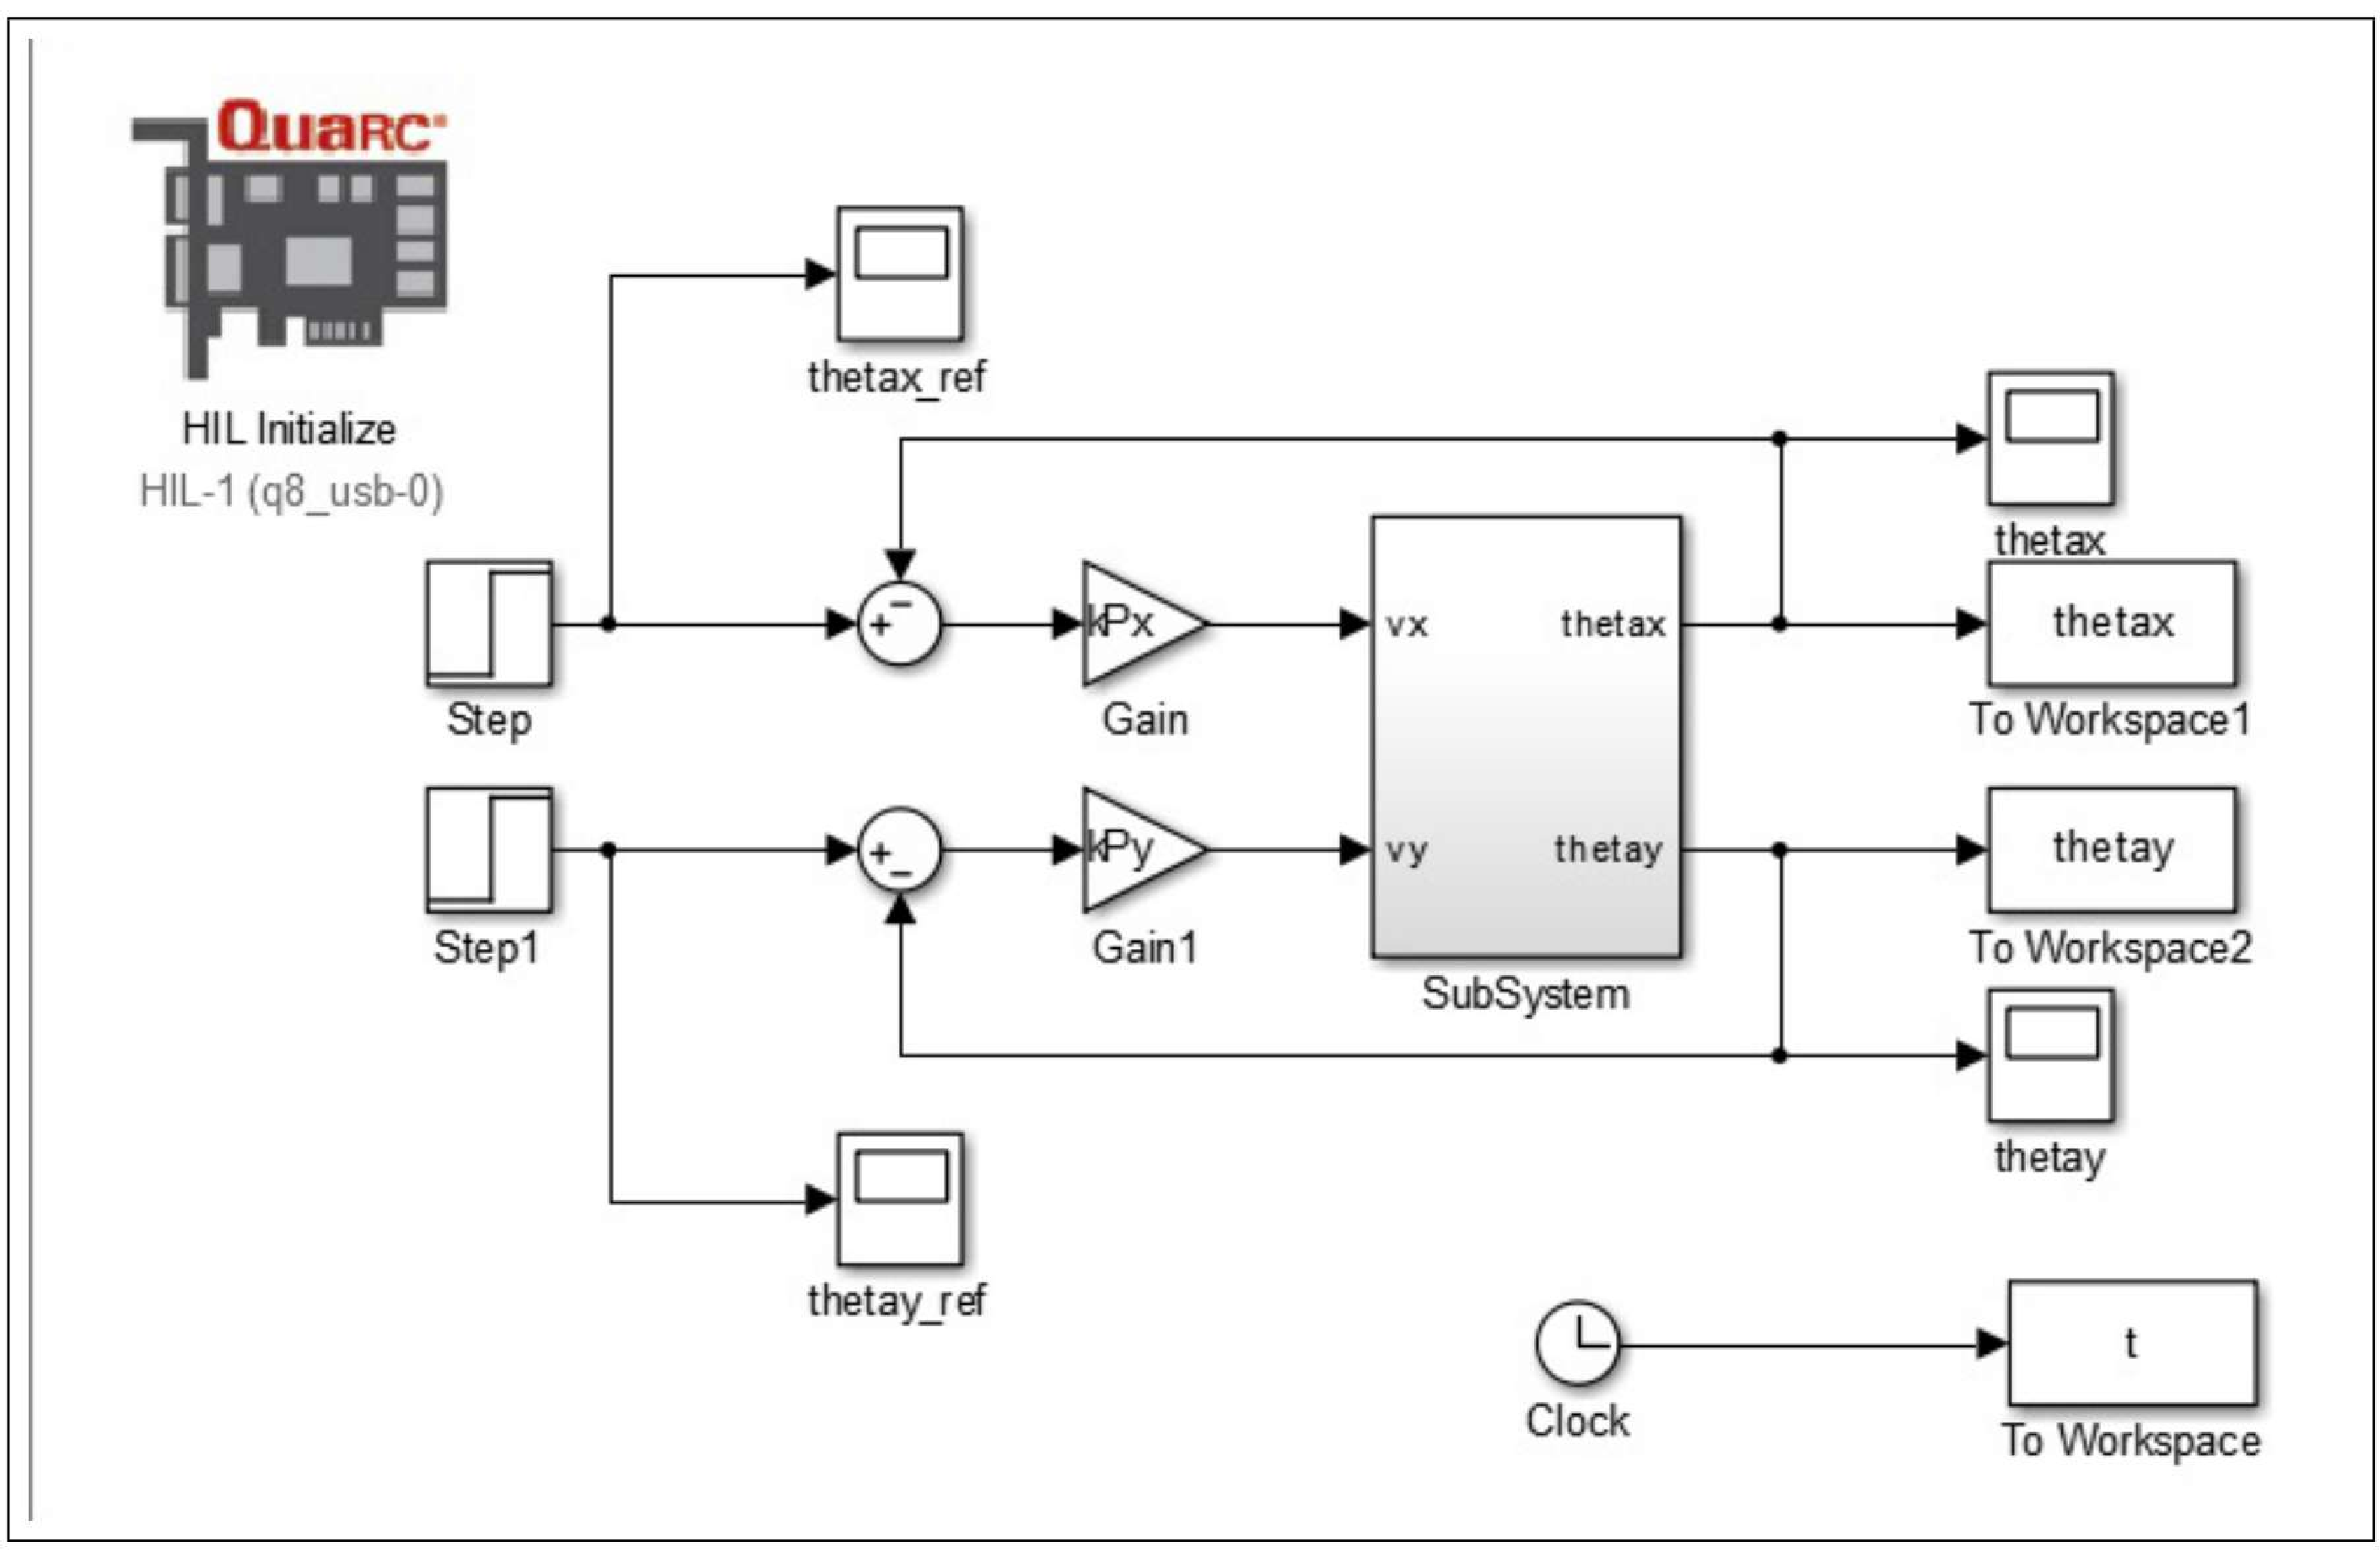
\includegraphics[width=0.9\linewidth]{figure/step2_model.pdf}
    \caption{P 制御の Simulink モデル(実機実験モデル ``\texttt{ex\_P.slx}'')}
    \label{fig:simulink_model_p}
\end{figure}

\vspace{1em}
\noindent
\textbf{ステップ 2}:
ステップ 1 の \texttt{\textyen ID} をカレントフォルダとして,実機実験モデル ``\texttt{ex\_P.slx}'' をコンパイルする.

\vspace{1em}
\noindent
\textbf{ステップ 2}:
ステップ1の \texttt{\textyen ID} をカレントフォルダとして,実機実験モデル ``\texttt{ex\_P.slx}'' をコンパイルする.

\vspace{1em}
\noindent
\textbf{ステップ 3}:
モータ軸の角度 $\theta_x(t)$ と $\theta_y(t)$ が $0$~[rad] となるように P 制御する.
実機実験モデル ``\texttt{ex\_P.slx}'' のブロック ``Step'',``Step1'' をダブルクリックし,

\[
\begin{array}{ll}
\text{Step}~(\theta_x^{\mathrm{ref}}(t))\!: &
\left\{
\begin{array}{l}
\text{ステップ時間: } 0 \\
\text{初期値: } 0 \\
\text{最終値: } 0 \\
\text{サンプル時間: } 0
\end{array}
\right., \quad
\text{Step1}~(\theta_y^{\mathrm{ref}}(t))\!: 
\left\{
\begin{array}{l}
\text{ステップ時間: } 0 \\
\text{初期値: } 0 \\
\text{最終値: } 0 \\
\text{サンプル時間: } 0
\end{array}
\right.
\end{array}
\]

のように変更して,モータ軸の目標角度 $\theta_x^{\mathrm{ref}}(t)$,$\theta_y^{\mathrm{ref}}(t)$ を設定する.
ターゲットに接続し,実行してアーム角度が $0$ になっていることを確認する.

\vspace{1em}
\noindent
\textbf{ステップ 4}:
実機実験モデル ``\texttt{ex\_P.slx}'' のブロック ``Step'',``Step1'' をダブルクリックし,

\[
\begin{array}{ll}
\text{Step}~(\theta_x^{\mathrm{ref}}(t))\!: &
\left\{
\begin{array}{l}
\text{ステップ時間: } 0 \\
\text{初期値: } 0 \\
\text{最終値: } 0.2 \\
\text{サンプル時間: } 0
\end{array}
\right., \quad
\text{Step1}~(\theta_y^{\mathrm{ref}}(t))\!: 
\left\{
\begin{array}{l}
\text{ステップ時間: } 0 \\
\text{初期値: } 0 \\
\text{最終値: } 0.2 \\
\text{サンプル時間: } 0
\end{array}
\right.
\end{array}
\]

のように変更して,モータ軸の目標角度 $\theta_x^{\mathrm{ref}}(t)$,$\theta_y^{\mathrm{ref}}(t)$ を設定する.
\vspace{1em}
\noindent
\textbf{ステップ 5}: MATLAB Command Window で M ファイル ``\texttt{idarm.m}'' を実行すると,

\begin{tabbing}
\hspace{1cm}\=\kill
\> \texttt{>> idarm} \\
\> \texttt{ax = 40.9262} \hspace{6cm} \texttt{a\_x = 40.9262} \\
\> \texttt{bx = 76.7858} \hspace{6cm} \texttt{b\_x = 76.7858} \\
\> \texttt{ay = 42.1695} \hspace{6cm} \texttt{a\_y = 42.1695} \\
\> \texttt{by = 75.7744} \hspace{6cm} \texttt{b\_y = 75.7744}
\end{tabbing}

\vspace{1em}
\noindent
ようになり,パラメータの同定値が計算される.また,図~\ref{fig:step_response2} に示すグラフが表示される.なお,図~\ref{fig:step_response} における実線は実験データ,破線は同定された値を用いたシミュレーションデータのプロットである.また,$a_x$,$b_x$,$a_y$,$b_y$ は \texttt{armpara.mat} に保存されている.

\begin{figure}[htbp]
    \centering
    \begin{subfigure}[b]{0.45\linewidth}
        \centering
        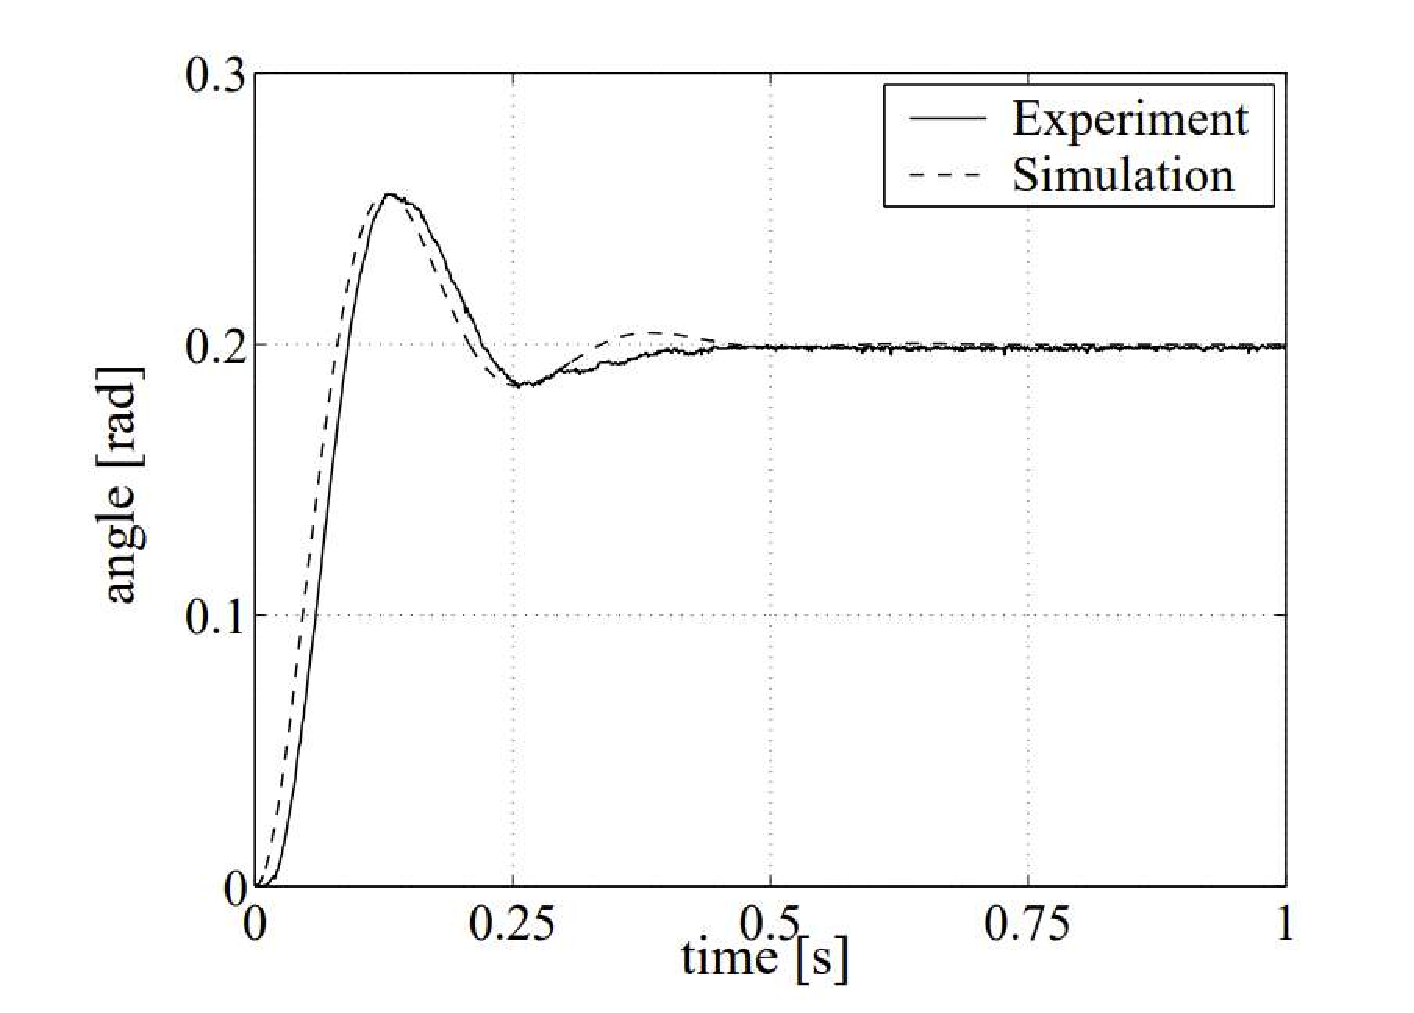
\includegraphics[width=\linewidth]{figure/thetax_response2.pdf}
        \caption{$\theta_x(t)$ の応答 ($\theta_x^{\mathrm{ref}}(t) = 0.2$, $\theta_y^{\mathrm{ref}}(t) = 0$)}
    \end{subfigure}
    \hfill
    \begin{subfigure}[b]{0.45\linewidth}
        \centering
        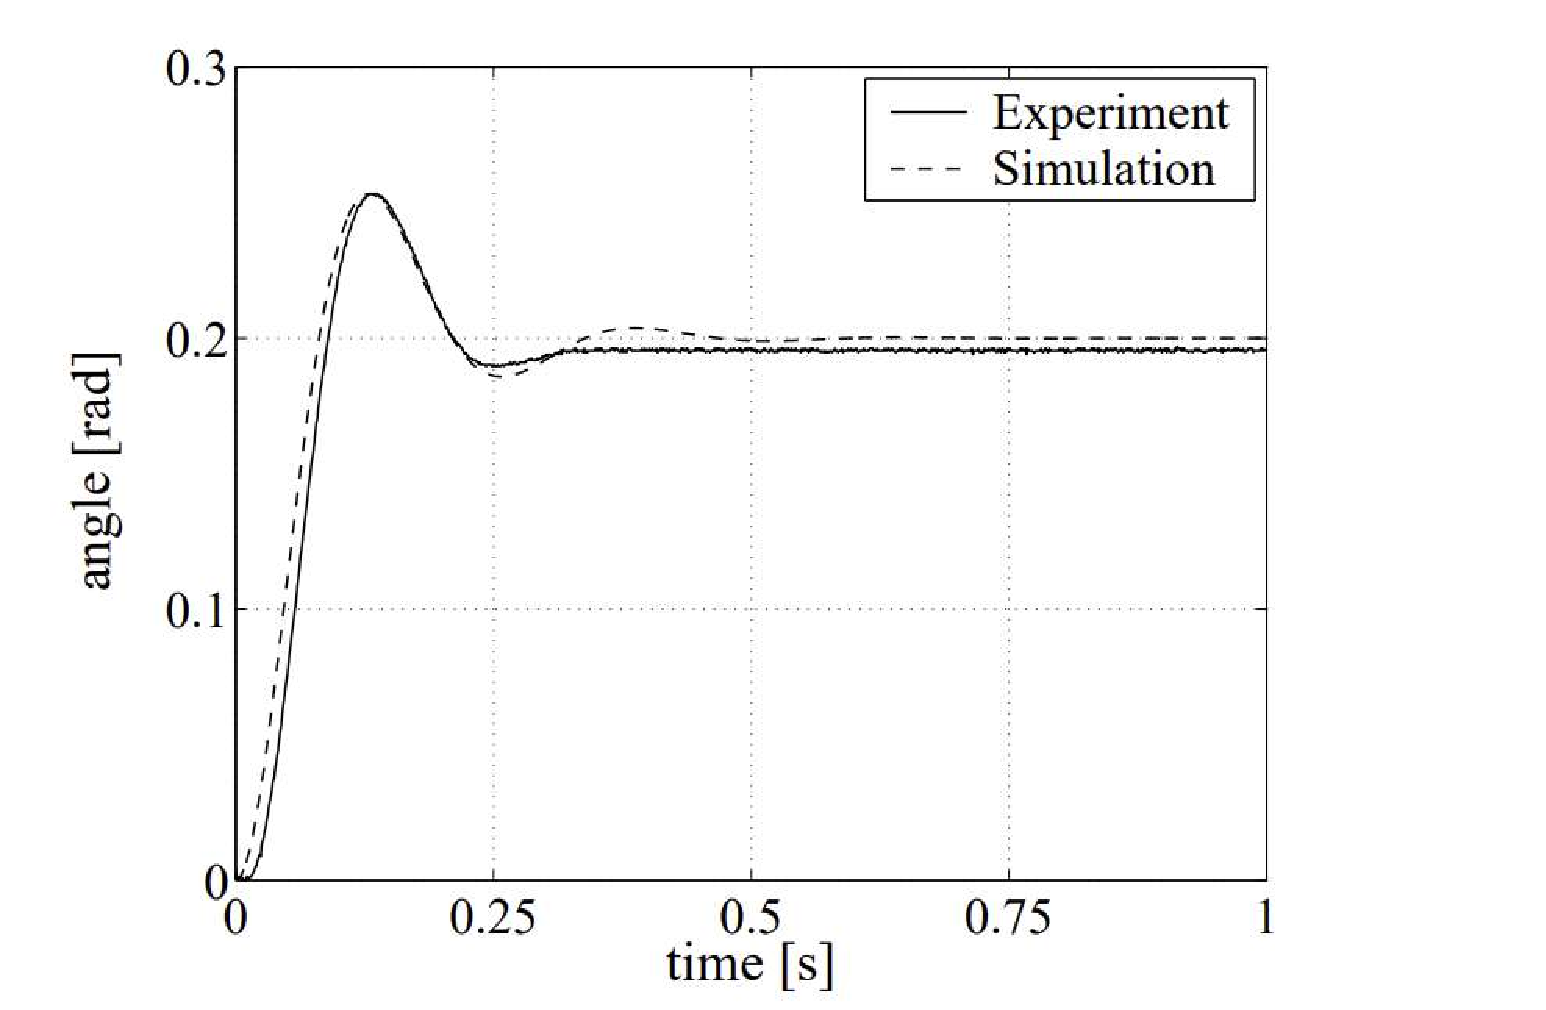
\includegraphics[width=\linewidth]{figure/thetay_response2.pdf}
        \caption{$\theta_y(t)$ の応答 ($\theta_x^{\mathrm{ref}}(t) = 0$, $\theta_y^{\mathrm{ref}}(t) = 0.2$)}
    \end{subfigure}
    \caption{P コントローラを用いたときのステップ応答 ($k_{Px}=20,\ k_{Py}=20$)}
    \label{fig:step_response2}
\end{figure}
 \newpage
% !TEX root = main.tex
\section{まとめ}

 \newpage
\section{手先位置制御}
\subsection{順運動学と逆運動学}

ここでは,手先位置 $(x(t), y(t))$ をその目標値 $(x^{\mathrm{ref}}(t), y^{\mathrm{ref}}(t))$ に追従させる制御を考える.

手先 $P_3$ の座標 $(x(t), y(t))$ を目標値 $(x^{\mathrm{ref}}(t), y^{\mathrm{ref}}(t))$ に追従させるためには,2.3 節で述べたように,逆運動学により角度の目標値 $\theta_x^{\mathrm{ref}}(t), \theta_y^{\mathrm{ref}}(t)$ を

\begin{equation}
\begin{cases}
\theta_x^{\mathrm{ref}}(t) = \sin^{-1} \left( \frac{\sqrt{x^{\mathrm{ref}}(t)^2 + y^{\mathrm{ref}}(t)^2}}{2\ell} \right) + \tan^{-1} \left( \frac{y^{\mathrm{ref}}(t)}{x^{\mathrm{ref}}(t)} \right) \\
\theta_y^{\mathrm{ref}}(t) = \sin^{-1} \left( \frac{\sqrt{(x^{\mathrm{ref}}(t)-2\ell)^2 + y^{\mathrm{ref}}(t)^2}}{2\ell} \right) - \tan^{-1} \left( \frac{x^{\mathrm{ref}}(t) - 2\ell}{y^{\mathrm{ref}}(t)} \right)
\end{cases}
\end{equation}

と設定すればよい.

\vspace{1em}
たとえば I--PD コントローラ(比例・微分先行型 PID コントローラ)

\begin{equation}
\begin{cases}
v_x(t) = -k_{Px} \theta_x(t) + \frac{k_{Ix}}{s} e_x(t) - k_{Dx} \frac{d\theta_x(t)}{dt} \\
v_y(t) = -k_{Py} \theta_y(t) + \frac{k_{Iy}}{s} e_y(t) - k_{Dy} \frac{d\theta_y(t)}{dt}
\end{cases}
\end{equation}

を用いると,$\theta_x(t), \theta_y(t)$ をその目標値に追従させることができ,その結果,2.2節で述べたように,順運動学により手先位置 $(x(t), y(t))$ は次式のようになる:

\begin{equation}
\begin{cases}
x(t) = h(t) \cos(\theta_x(t) - \alpha_x(t)) - \frac{d(t)}{2} \sin(\theta_x(t) - \alpha_x(t)) + \ell \sin \theta_x(t) \\
y(t) = h(t) \sin(\theta_x(t) - \alpha_x(t)) + \frac{d(t)}{2} \cos(\theta_x(t) - \alpha_x(t)) - \ell \cos \theta_x(t)
\end{cases}
\end{equation}

ただし,

\begin{equation}
\begin{cases}
d(t) = \sqrt{(p_{2x}(t) - p_{4x}(t))^2 + (p_{2y}(t) - p_{4y}(t))^2} \\
h(t) = \sqrt{\ell^2 - \left( \frac{d(t)}{2} \right)^2} \\
\alpha_x(t) = \cos^{-1} \left( \frac{\ell^2 + d(t)^2 - (p_{4x}(t)^2 + p_{4y}(t)^2)}{2\ell d} \right) \\
p_{2x}(t) = \ell \sin \theta_x(t),\quad p_{2y}(t) = -\ell \cos \theta_x(t) \\
p_{4x}(t) = 2\ell - \ell \cos \theta_y(t),\quad p_{4y}(t) = -\ell \sin \theta_y(t)
\end{cases}
\end{equation}

である.

図~\ref{fig:block_diagram} に手先位置 $(x(t), y(t))$ をその目標値 $(x^{\mathrm{ref}}(t), y^{\mathrm{ref}}(t))$ に追従させるフィードバック制御系のブロック線図を示す.

\begin{figure}[H]
  \centering
  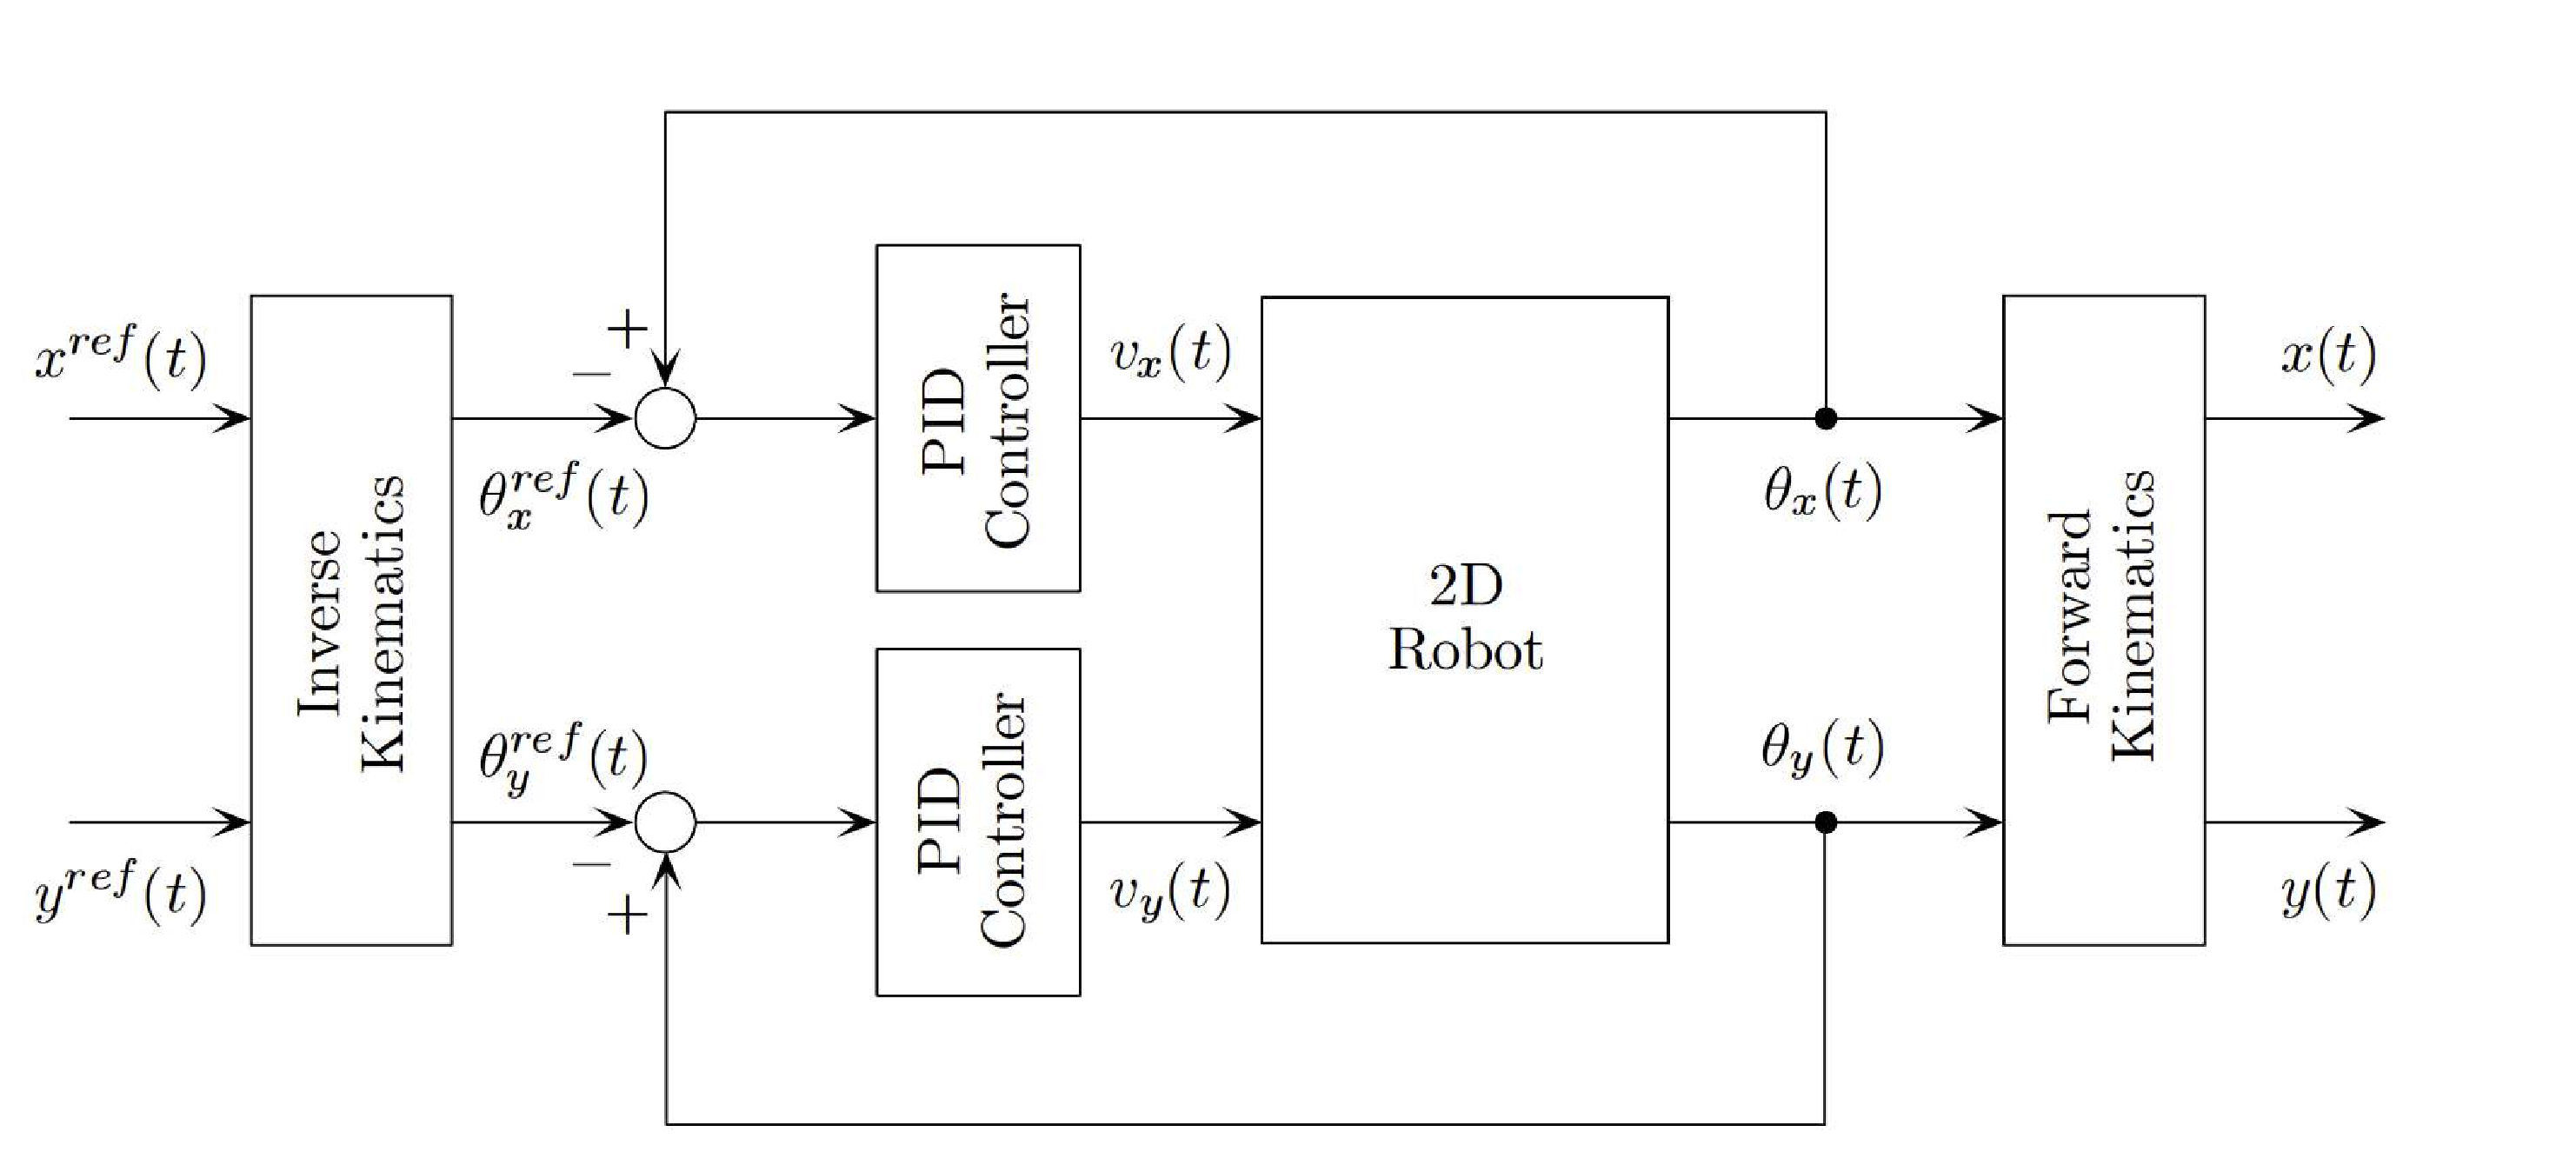
\includegraphics[width=0.85\linewidth]{figure/block6_1.pdf}
  \caption{フィードバック制御系}
  \label{fig:block_diagram}
\end{figure}

\subsection{シミュレーションと実験(目標値が一定値の場合)}

\fbox{\textbf{ステップ 1}}:
5.1.2 節で示した ``armpara.m'',5.3.2 節で示した ``armIPD.m'' およびシミュレーション結果をアニメーション表示する以下の M ファイル ``sim\_anime.m'' を作成し,\textbackslash xy に保存する.
また,シミュレーションモデル ``sim\_robot\_xy.slx''(図~\ref{fig:sim_robot_xy}(a)),実機実験モデル ``ex\_robot\_xy.slx''(図~\ref{fig:sim_robot_xy}(b))を作成し,\textbackslash xy に保存する.ただし,各 \texttt{Subsystem} の内容は以下に示すとおりである.

\begin{figure}[H]
    \centering
    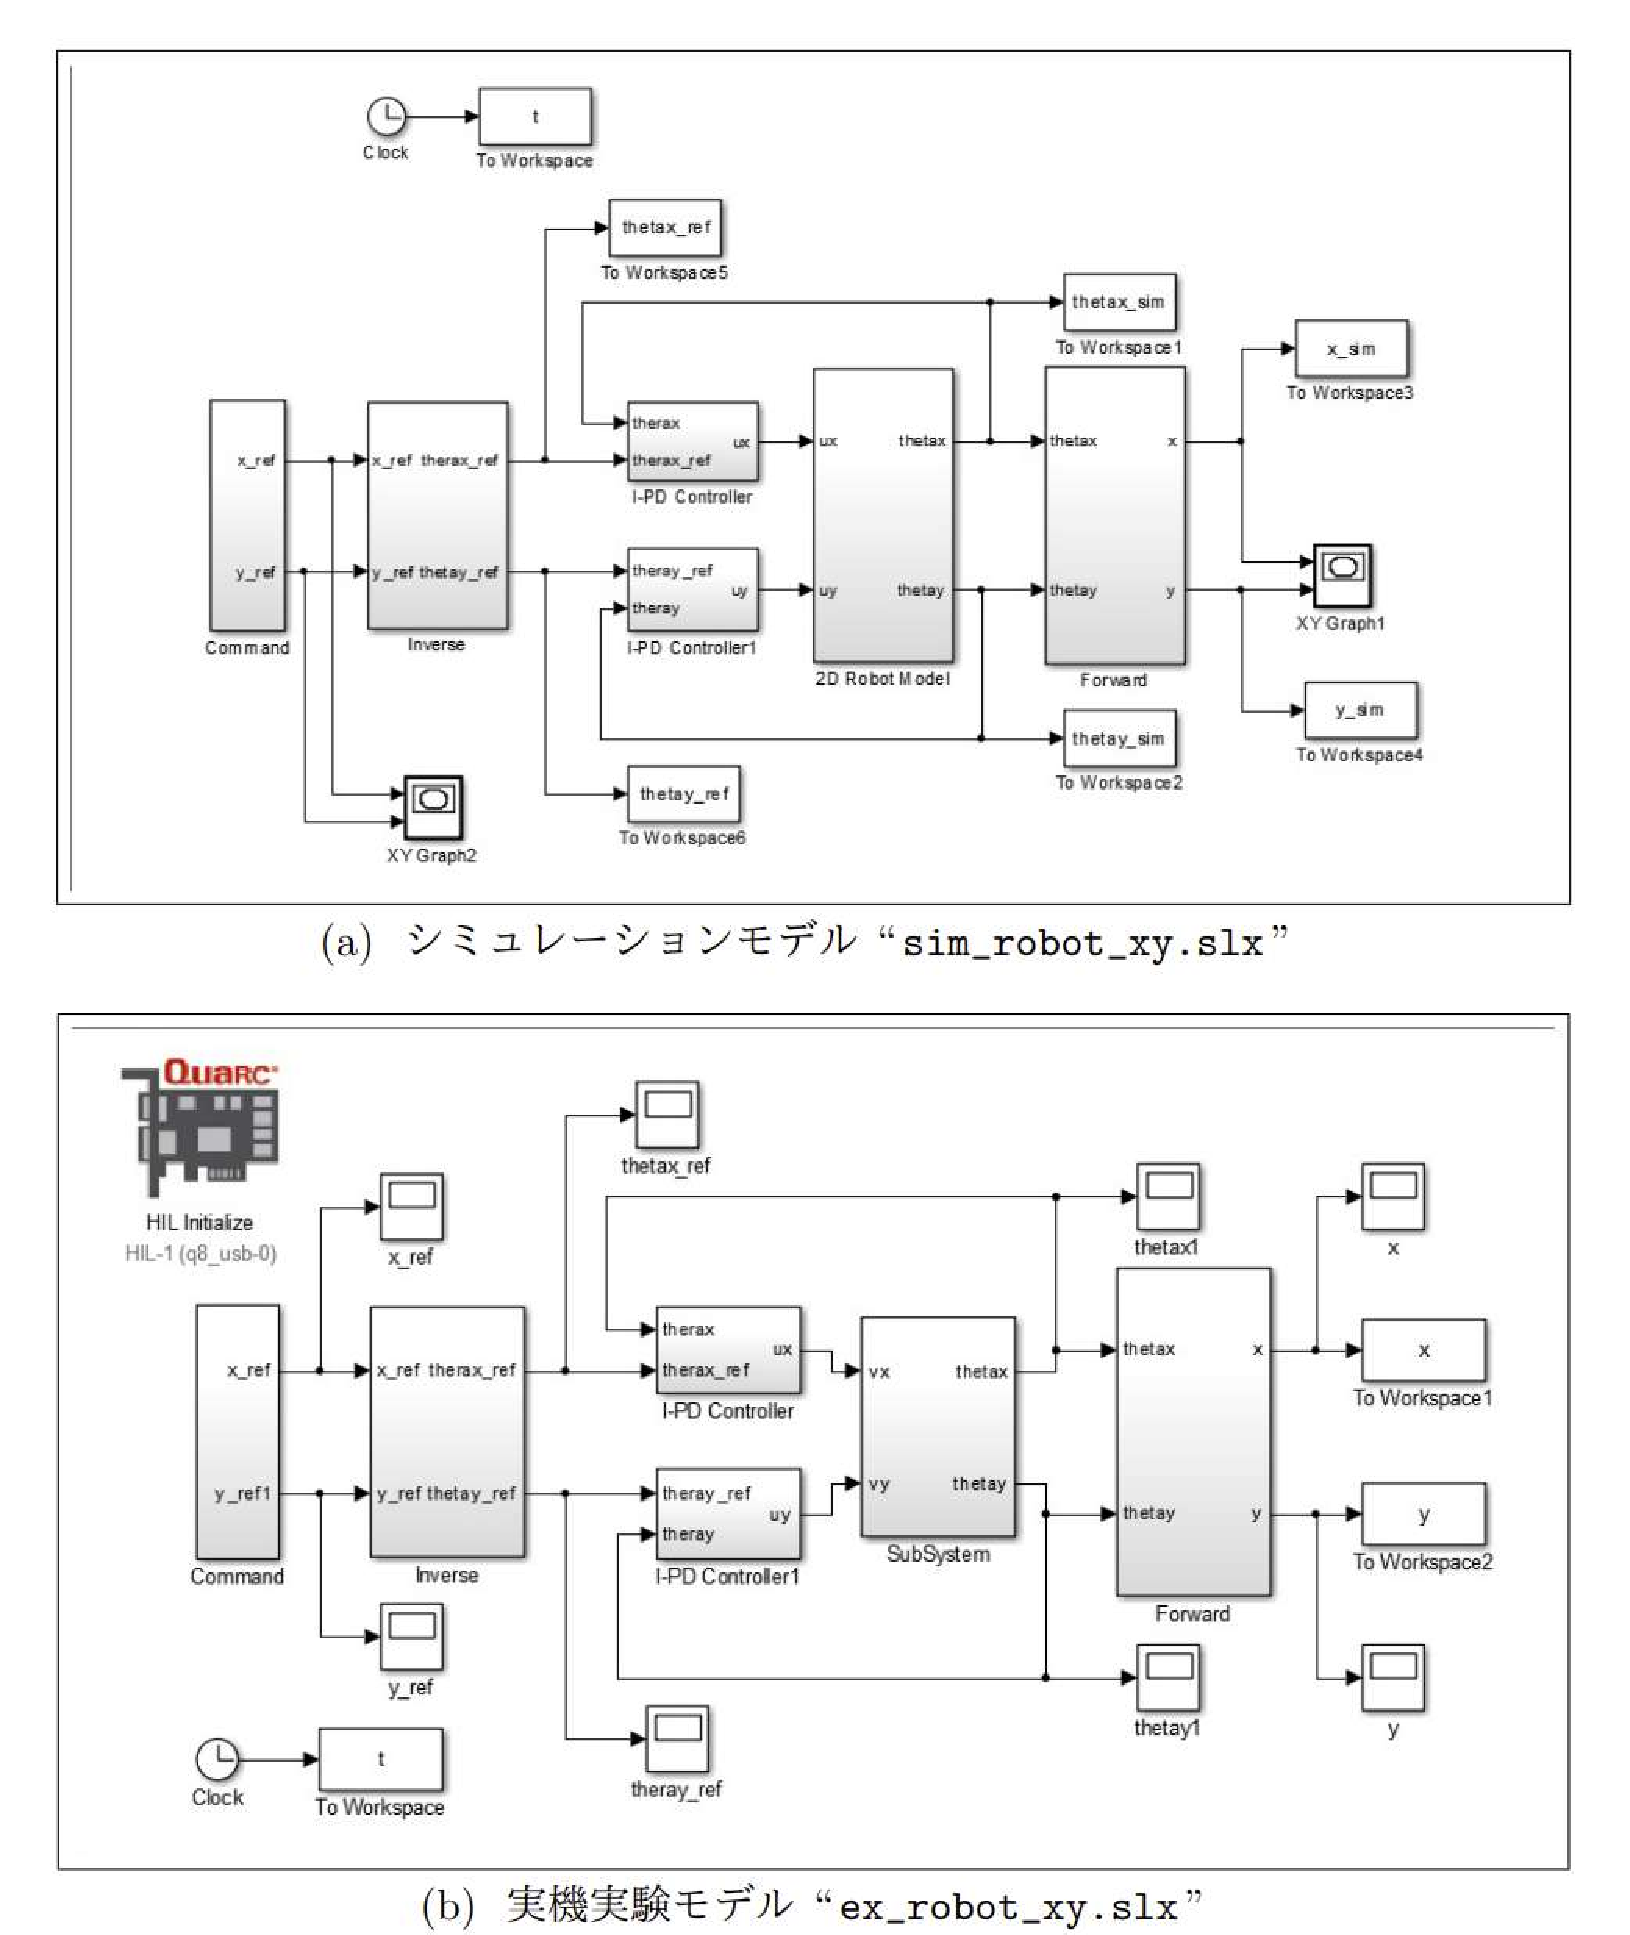
\includegraphics[width=0.85\linewidth]{figure/robot_xy_models.pdf}
    \caption{手先位置制御(目標値が一定値の場合)}
    \label{fig:sim_robot_xy}
\end{figure}

\begin{figure}[H]
    \centering
    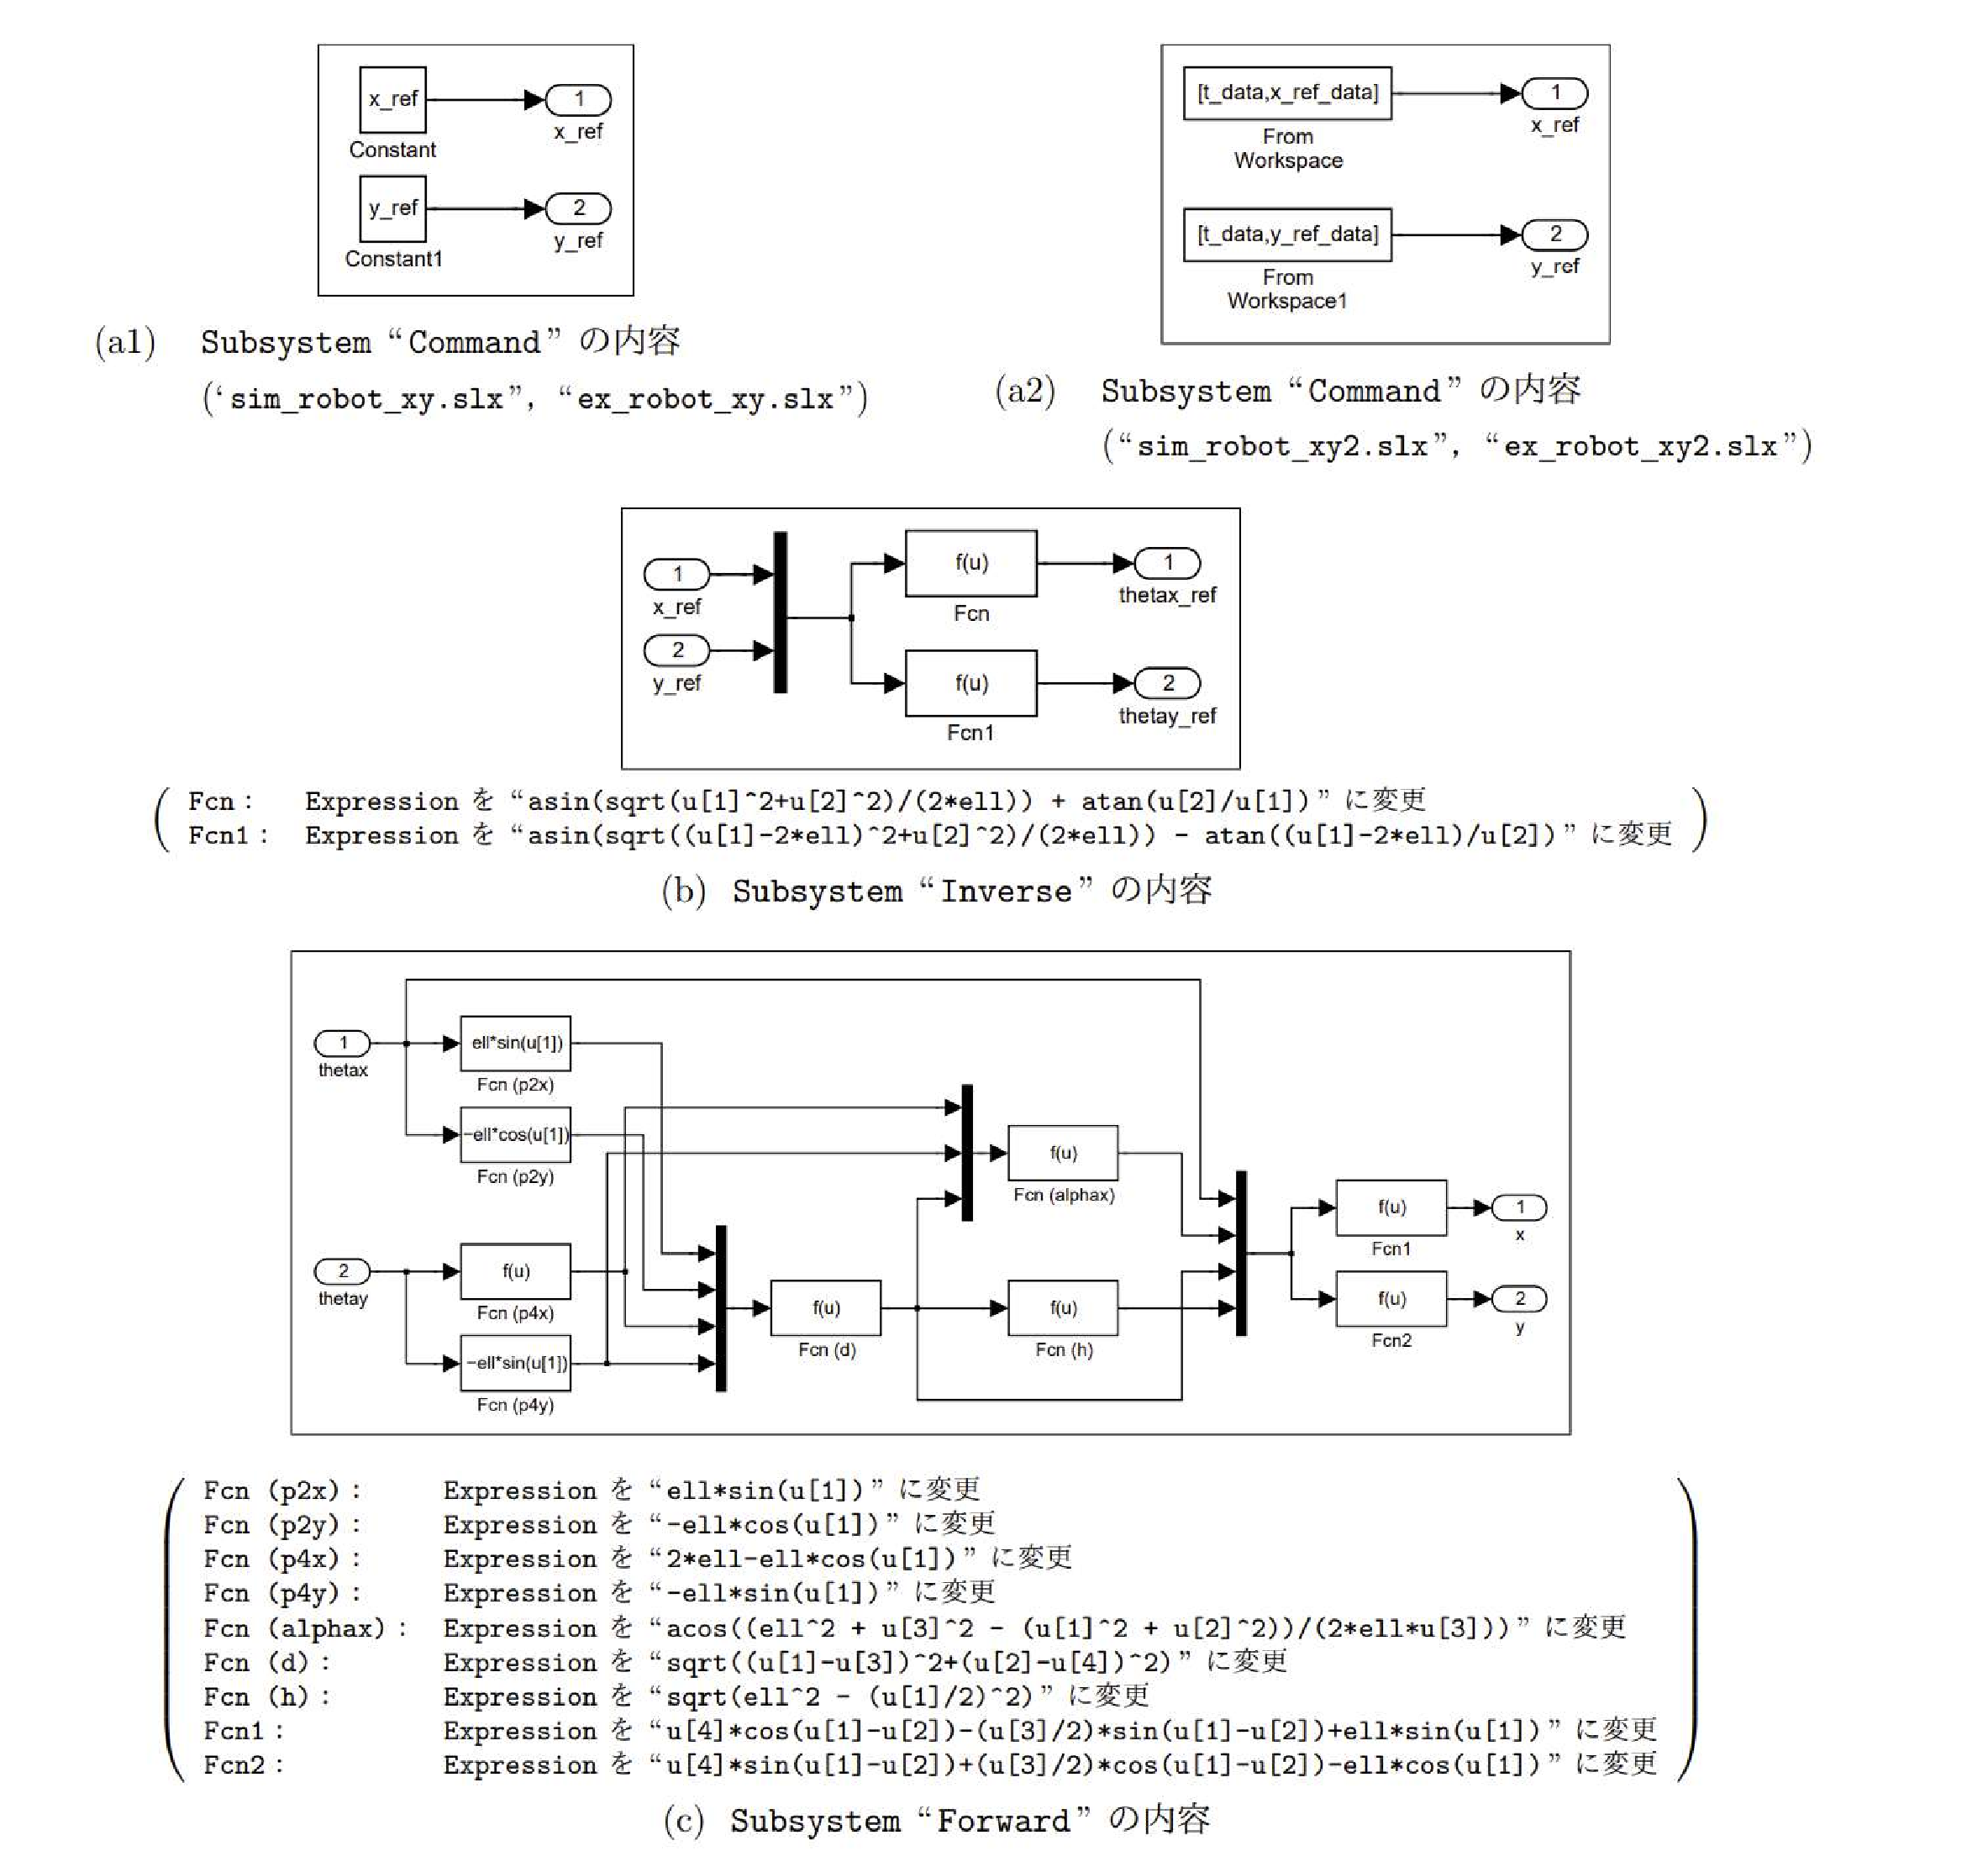
\includegraphics[width=1.0\linewidth]{figure/subsystem_all.pdf}
    \caption{Subsystem ``Command'', ``Inverse'', ``Forward'' の構成(図~6.3)}
    \label{fig:subsystems}
\end{figure}

\fbox{\textbf{ステップ 2}}: まず,MATLAB Command Window で
\begin{verbatim}
>> armIPD
各パラメータを設定して下さい
omegaMx = 20
omegaMy = 20
  …(略)…
alphaM1x = 2
alphaM2x = 2
alphaM1y = 2
alphaM2y = 2
  …(略)…
x_ref = 0.15; y_ref = -0.05;
\end{verbatim}

と入力し,パラメータを設定する.つぎに,シミュレーションを開始し,シミュレーション終了後に以下のように入力して結果をアニメーション表示する.
\begin{verbatim}
>> sim_anime;
\end{verbatim}

アニメーション(図~\ref{fig:xy_animation}~(a))によって各リンクに無理な動きがないことを確認した後,``ex\_robot\_xy.slx''をコンパイルしてから実機実験を行うと,図~\ref{fig:xy_animation}~(b) の実験結果が得られる.

\begin{figure}[H]
    \centering
    \begin{subfigure}[b]{0.45\linewidth}
        \centering
        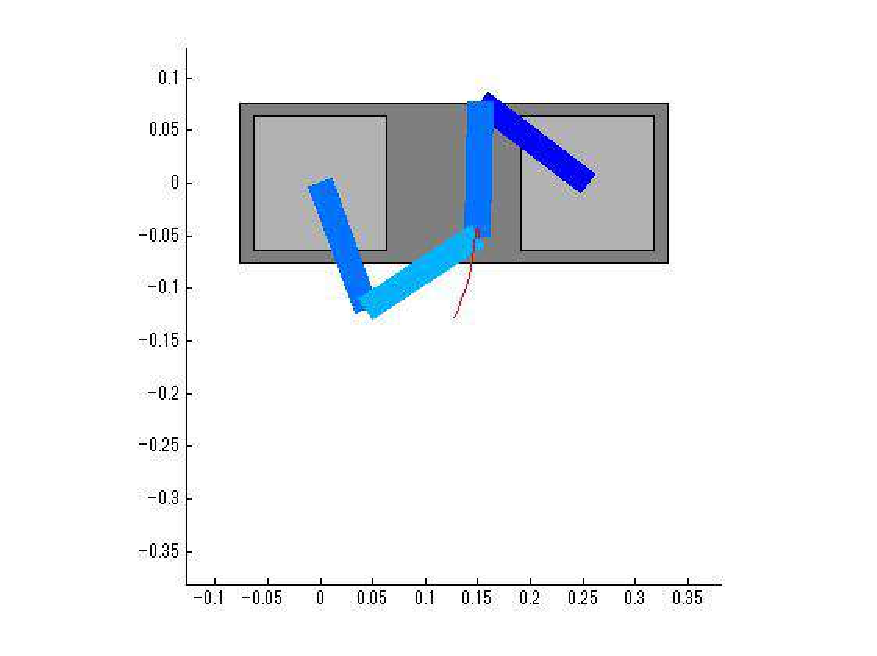
\includegraphics[width=\linewidth]{figure/sim_anime.pdf}
        \caption{シミュレーション結果のアニメーション表示}
    \end{subfigure}
    \begin{subfigure}[b]{0.45\linewidth}
        \centering
        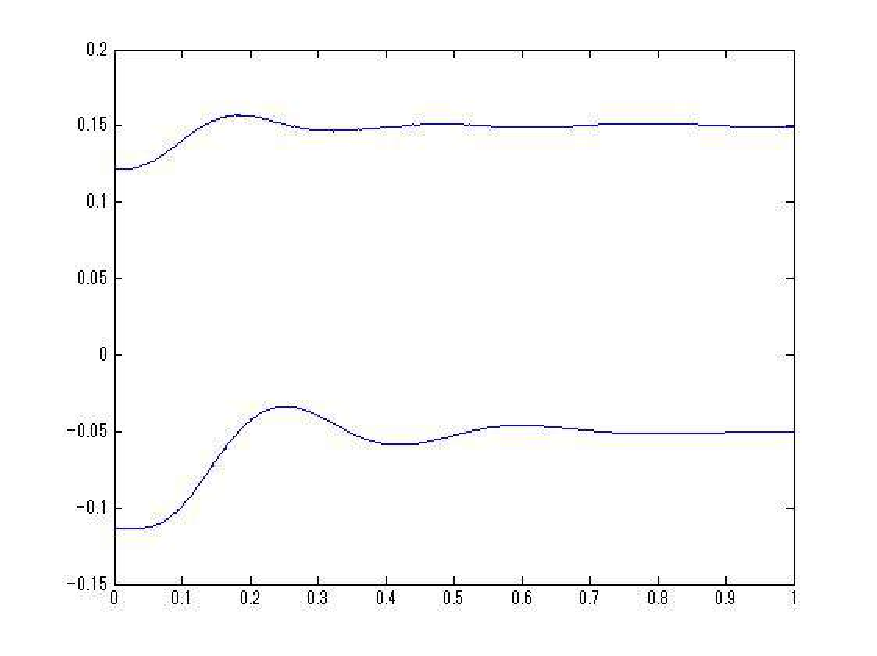
\includegraphics[width=\linewidth]{figure/ex_robot_guraf.pdf}
        \caption{実験結果}
    \end{subfigure}
    \caption{手先位置制御($x^{\mathrm{ref}}=0.15\ \mathrm{[m]}$, $y^{\mathrm{ref}}=-0.05\ \mathrm{[m]}$)}
    \label{fig:xy_animation}
\end{figure}

\subsection{シミュレーションと実験 (目標値をデータで与える場合)}
\subsubsection{目標値の与え方}
ここでは,目標値を以下のようにデータ列で与え,手先位置制御を行うことを考える.

\begin{lstlisting}[language=Matlab]
t_data       = [0; 1; 2; 3; 4];
x_ref_data   = [0.1; 0.2; 0.2; 0.1; 0.1];
y_ref_data   = [-0.15; -0.15; -0.05; -0.05; -0.15];
\end{lstlisting}

なお,このようにデータ列で目標値を与えたとき,図\ref{fig:xy_ref_data}のようになる.

\begin{figure}[H]
    \centering
    \begin{subfigure}[b]{0.45\linewidth}
        \centering
        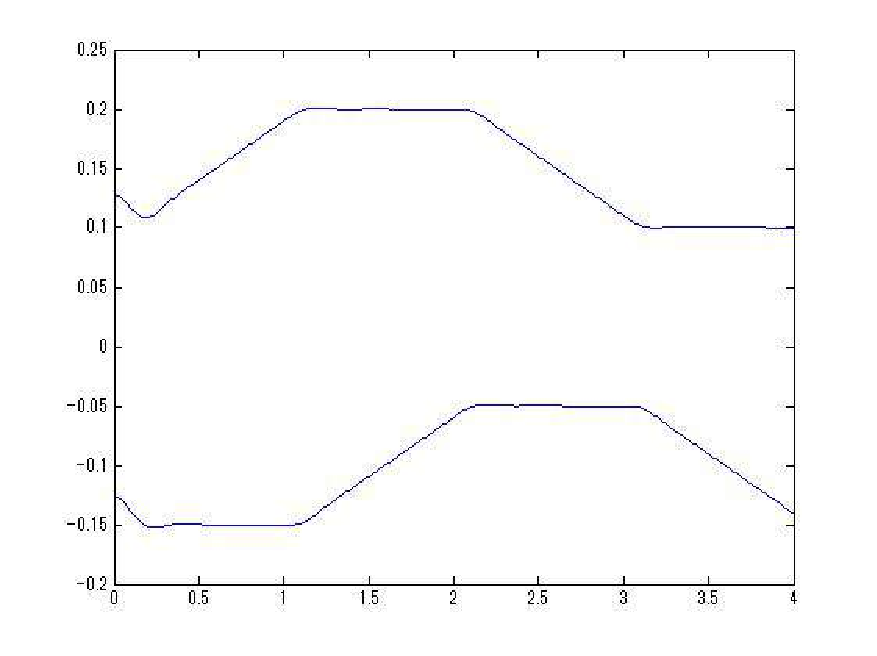
\includegraphics[width=\linewidth]{figure/sim_anime_2_grafu.pdf}
        \caption{$x^{\mathrm{ref}}(t)$ と $y^{\mathrm{ref}}(t)$}
    \end{subfigure}
    \begin{subfigure}[b]{0.45\linewidth}
        \centering
        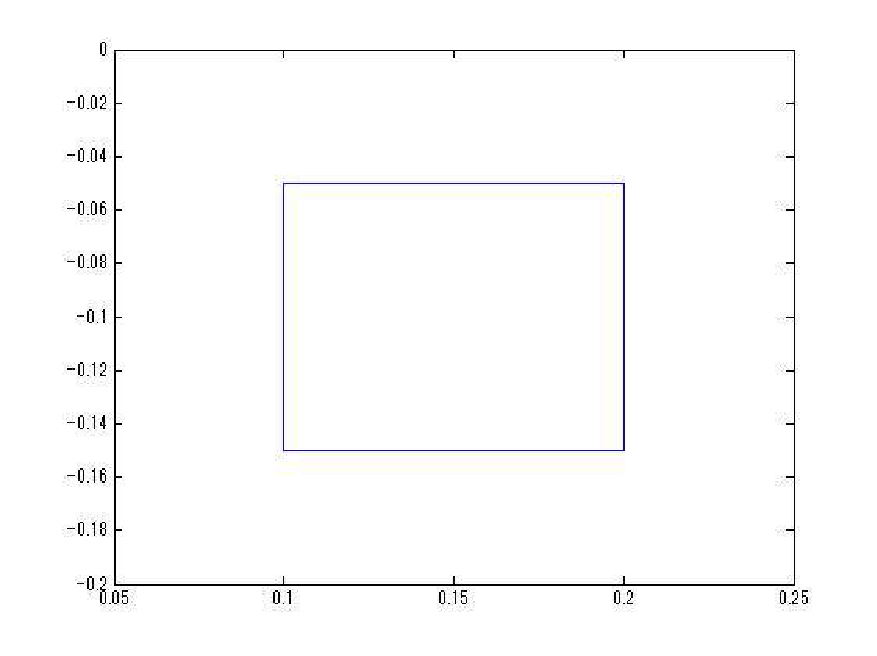
\includegraphics[width=\linewidth]{figure/sim_anime_2.pdf}
        \caption{$y^{\mathrm{ref}}$ vs $x^{\mathrm{ref}}$}
    \end{subfigure}
    \caption{データ列で与えられた手先の目標位置}
    \label{fig:xy_ref_data}
\end{figure}

\subsubsection{デモンストレーション}

ここでは,花の絵を描くような目標位置データを用いた手先位置制御のデモンストレーションを行う.
このデータは M ファイル ``flower\_data.m'' に含まれており,$(x^{\mathrm{ref}}(t), y^{\mathrm{ref}}(t))$ の時系列データとして定義されている.
この目標位置に追従する様子をアニメーション表示するために,MATLAB Command Window で以下のように入力する.

\begin{lstlisting}[language=Matlab]
flower_data                                % flower_data.m の実行(手先位置の目標値設定)
figure(1); plot(t_data,x_ref_data); 
xlabel('time [s]'); ylabel('x^{ref} [m]'); % (t, x_ref(t)) のプロット
figure(2); plot(t_data,y_ref_data); 
xlabel('time [s]'); ylabel('y^{ref} [m]'); % (t, y_ref(t)) のプロット
figure(3); plot(x_ref_data,y_ref_data);    % (x_ref(t), y_ref(t)) のプロット
xlabel('x^{ref} [m]'); ylabel('y^{ref} [m]');
t = t_data; x = x_ref_data; y = y_ref_data;
figure(4); sim_anime                       % flower_anime.m の実行(アニメーション)
\end{lstlisting}

ここでは,M ファイル ``flower\_data.m'' に含まれている花の絵のような目標位置データを用いて,手先位置制御の動作をデモンストレーションする.
このファイルには,時系列で与えられた手先の目標位置 $(x^{\mathrm{ref}}(t), y^{\mathrm{ref}}(t))$ が含まれており,それを基にアニメーション表示およびグラフ出力を行う.
MATLAB Command Window で以下のように入力すればよい.

\begin{lstlisting}[language=Matlab]
flower_data                                % flower_data.m の実行(手先位置の目標値設定)
figure(1); plot(t_data,x_ref_data); 
xlabel('time [s]'); ylabel('x^{ref} [m]'); % (t, x_ref(t)) のプロット
figure(2); plot(t_data,y_ref_data); 
xlabel('time [s]'); ylabel('y^{ref} [m]'); % (t, y_ref(t)) のプロット
figure(3); plot(x_ref_data,y_ref_data);    % (x_ref(t), y_ref(t)) のプロット
xlabel('x^{ref} [m]'); ylabel('y^{ref} [m]');
t = t_data; x = x_ref_data; y = y_ref_data;
figure(4); sim_anime                       % flower_anime.m の実行(アニメーション)
\end{lstlisting}

その結果,図\ref{fig:xy_flower} に示すような時系列グラフおよびアニメーション表示が得られる.

\begin{figure}[H]
    \centering
    \begin{subfigure}[b]{0.45\linewidth}
        \centering
        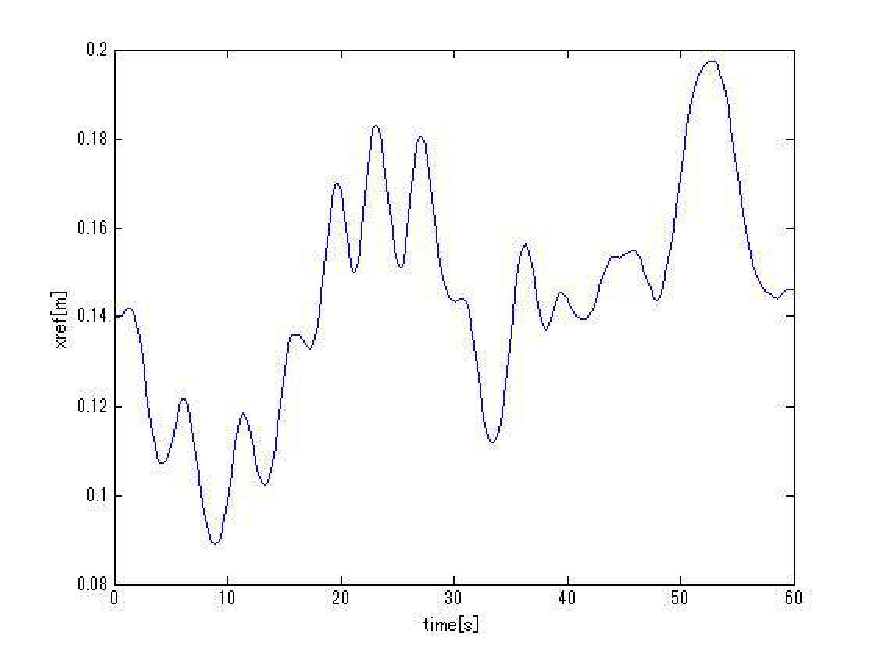
\includegraphics[width=\linewidth]{figure/xref.pdf}
        \caption{$x^{\mathrm{ref}}(t)$}
    \end{subfigure}
    \begin{subfigure}[b]{0.45\linewidth}
        \centering
        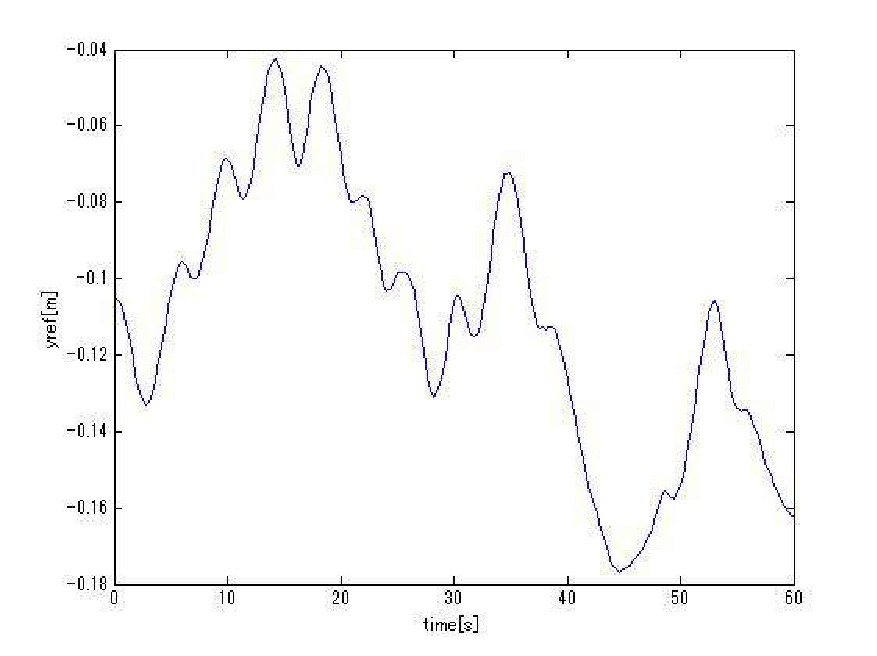
\includegraphics[width=\linewidth]{figure/yref.pdf}
        \caption{$y^{\mathrm{ref}}(t)$}
    \end{subfigure}

    \begin{subfigure}[b]{0.45\linewidth}
        \centering
        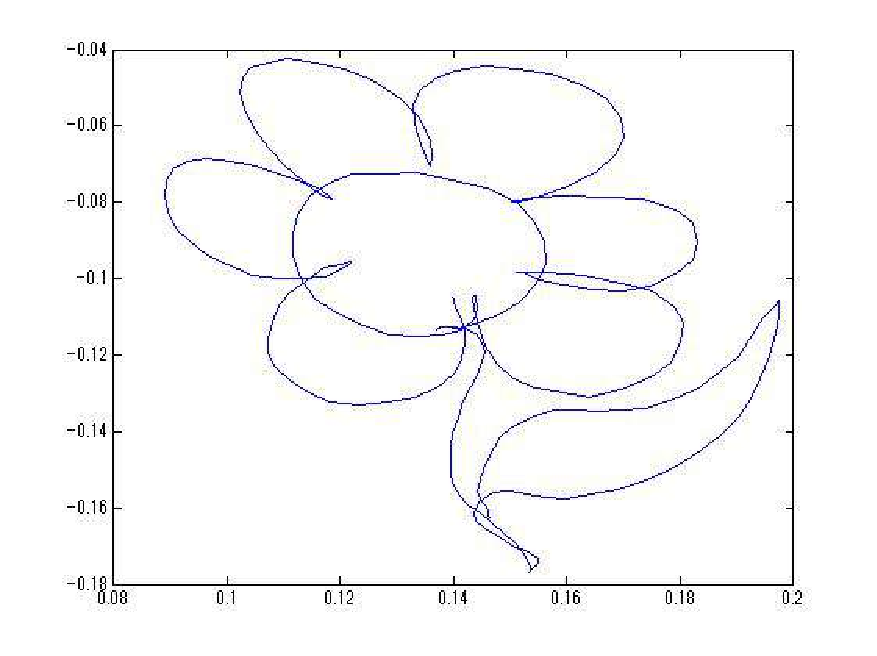
\includegraphics[width=\linewidth]{figure/mokuhyoukidou.pdf}
        \caption{目標軌道}
    \end{subfigure}
    \begin{subfigure}[b]{0.45\linewidth}
        \centering
        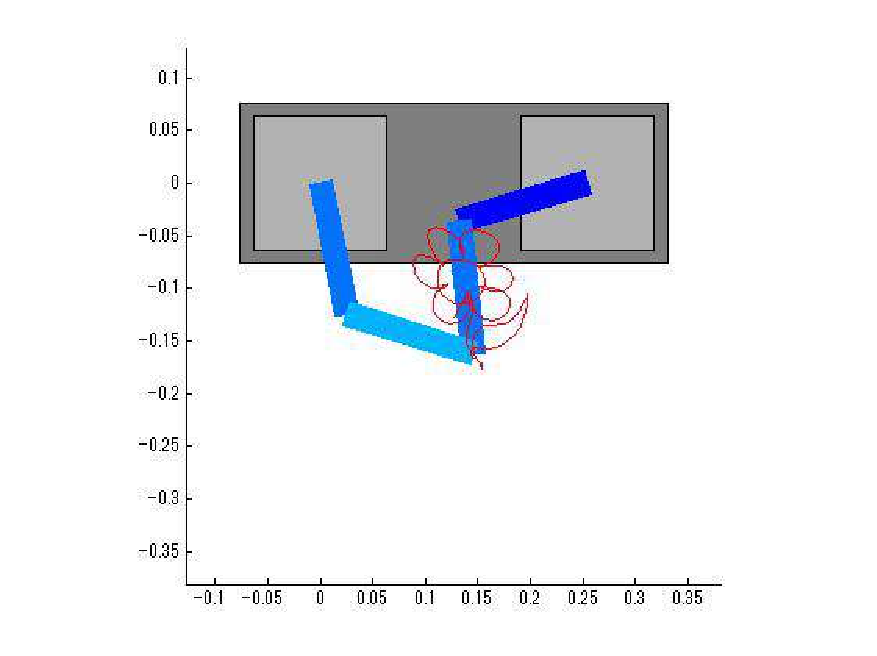
\includegraphics[width=\linewidth]{figure/fig4_sim_anime.pdf}
        \caption{アニメーション表示}
    \end{subfigure}
    \caption{\texttt{flower\_data.m} により設定された手先の目標位置}
    \label{fig:xy_flower}
\end{figure}

この花の絵の目標値データを利用して実験を行うために,MATLAB Command Window で以下のように入力
し,パラメータ設定を行う.
\begin{lstlisting}[language=Matlab]
    armIPD
    各パラメータを設定して下さい
    omegaMx = 20
    omegaMy = 20
    ........................................................... 《略》 ...........................................................
    alphaM1x = 2
    alphaM2x = 2
    alphaM1y = 2
    alphaM2y = 2
    ........................................................... 《略》 ...........................................................
    flower_data   % flower_data.m の実行(手先位置の目標値設定)
\end{lstlisting}
つぎに,``sim\_robot\_xy2.slx'' によりシミュレーションを実行する.
M ファイル \texttt{sim\_anime} を実行してアニメーションで各リンクに無理な動きがないことを確認した後,
``ex\_robot\_xy2.slx'' をコンパイルしてから実機実験を行うと,図\ref{fig:xy_flower_result} の実験結果が得られる.

\begin{figure}[H]
    \centering
    \begin{subfigure}[b]{0.45\linewidth}
        \centering
        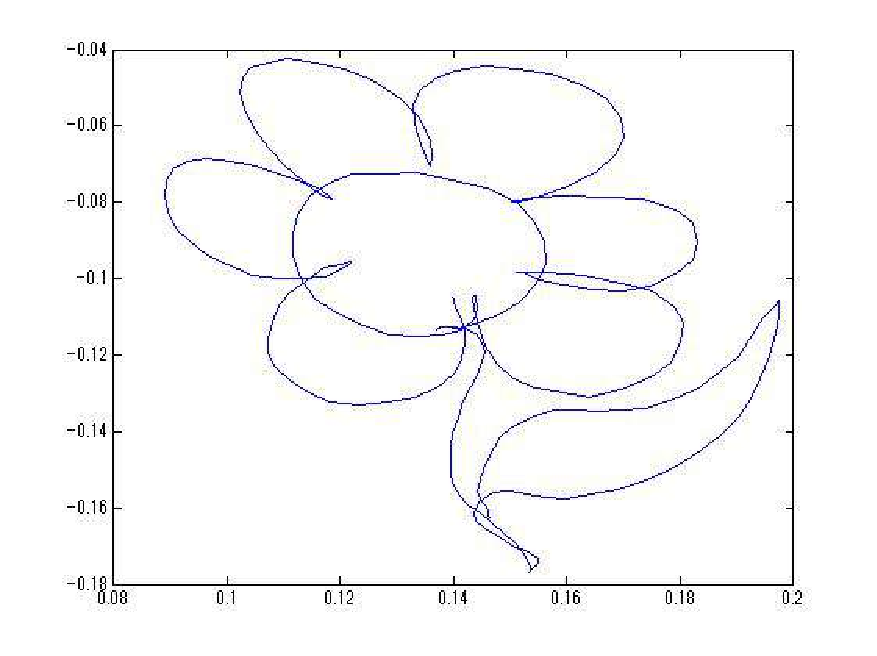
\includegraphics[width=\linewidth]{figure/mokuhyouchi.pdf}
        \caption{目標軌道}
    \end{subfigure}
    \begin{subfigure}[b]{0.45\linewidth}
        \centering
        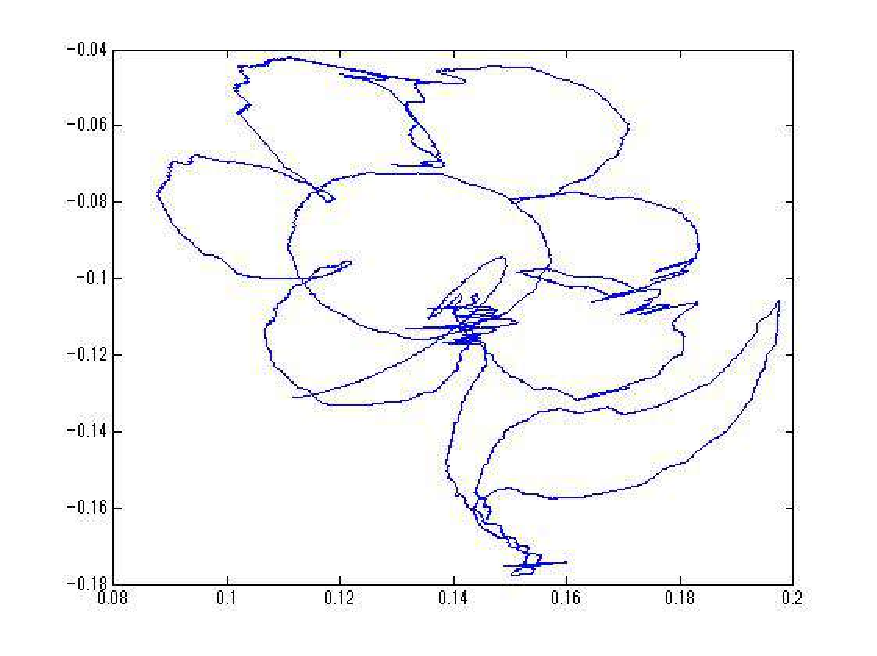
\includegraphics[width=\linewidth]{figure/zikkennkekka.pdf}
        \caption{実験結果}
    \end{subfigure}
    \caption{手先位置制御}
    \label{fig:xy_flower_result}
\end{figure}
 \newpage
% !TEX root = main.tex \newpage

%%%%%%%%%%%%%%%%%%%%%%%%%%%%%%%%%%%%%%%%%%%%%%%%%%%%%%%%%%%%%%%%%%%%%%%%%%%%%
%%%%%% 参考文献 %%%%%%%%%%%%%%%%%%%%%%%%%%%%%%%%%%%%%%%%%%%%%%%%%%%%%%%%%%%
%%%%%%%%%%%%%%%%%%%%%%%%%%%%%%%%%%%%%%%%%%%%%%%%%%%%%%%%%%%%%%%%%%%%%%%%%%%%%
% !TEX root = main.tex
%%%%%%%%%%%%%%%%%%%%%%%%%%%%%%%%%%%%%%%%%%%%%%%%%%%%%%%%%%%%%%%%%%%%%%%%
\begin{center}
	\section*{\kintou{5zw}{参考文献}}                      %% ここに番号をつけない
	\vspace*{-2zh}
\end{center}
\addcontentsline{toc}{section}{参考文献} %% 目次に番号をつけない
%%%%%%%%%%%%%%%%%%%%%%%%%%%%%%%%%%%%%%%%%%%%%%%%%%%%%%%%%%%%%%%%%%%%%%%%

\begin{thebibliography}{99}
	
	\bibitem{nougyou}
	唐橋 需
	:農業用ロボットへの期待, 
	農業機械学会誌  57 巻 6 号 pp.145-150 (2021)
	
	\bibitem{nougyouziritu}
	有山 達也,伊藤 和寿
	:農業用搬送台車の自立移動における課題と開発事例, 
	システム/制御/情報 Vol.65,No.12,pp.489-494 (2021)
	
	\bibitem{saga-u}
	佐賀大学プレスリリース:
	カメラ映像のみで経路を自律走行するロボット車両を開発, 
	\url{https://www.saga-u.ac.jp/koho/press/2021120623170}, 
	[Accessed: Dec. 25, 2024].
	
	\bibitem{hirei}
	伊藤,阿部,今西,奥野,辻,三宅:
	比例航法を用いた自立移動ロボットの誘導,
	学術講演会前刷集No.76-10 368-20105161,
	
	P13 (2010)
	\bibitem{roshon}
	出村 公成, 萩原 良信, 升谷 保博, タン ジェフリー トゥ チュアン
	:ROS2とPythonで作って学ぶAIロボット入門, 
	講談社 (2018)
	
	\bibitem{realsense}
	インテル® RealSense™ デプスカメラ D435i /
	: \url{https://www.intel.co.jp/content/www/jp/ja/products/sku/190004/intel-realsense-depth-camera-d435i/specifications.html}, [Accessed: Dec. 25, 2024].
	
	\bibitem{stm}
	STM32 Nucleo-64: \url{https://www.st.com/ja/evaluation-tools/nucleo-f446re.html}, [Accessed: Dec. 25, 2024].
	
	\bibitem{amt}
	AMT102: \url{https://www.sameskydevices.com/product/resource/amt10e-v.pdf}, [Accessed: Dec. 25, 2024].
	
	\bibitem{ros2design}
	ROS 2 Design Documents: \url{https://design.ros2.org/}, [Accessed: Dec. 25, 2024].
	
	\bibitem{ros2docs}
	ROS 2 Documentation: \url{https://docs.ros.org/en/humble/index.html}, [Accessed: Dec. 25, 2024].
	
	\bibitem{yolo}
	ultralytics: \url{https://docs.ultralytics.com/ja/yolov5/}, [Accessed: Dec. 25, 2024].
	
\end{thebibliography}
% ******************************************* \newpage

%%%%%%%%%%%%%%%%%%%%%%%%%%%%%%%%%%%%%%%%%%%%%%%%%%%%%%%%%%%%%%%%%%%%%%%%%%%%%
%%%%%% 謝辞 %%%%%%%%%%%%%%%%%%%%%%%%%%%%%%%%%%%%%%%%%%%%%%%%%%%%%%%%%%%%%%%
%%%%%%%%%%%%%%%%%%%%%%%%%%%%%%%%%%%%%%%%%%%%%%%%%%%%%%%%%%%%%%%%%%%%%%%%%%%%%
%% !TEX root = main.tex
%%%%%%%%%%%%%%%%%%%%%%%%%%%%%%%%%%%%%%%%%%%%%%%%%%%%%%%%%%%%%%%%%%%%%%%%
\begin{center}
    \section*{\kintou{2.5zw}{謝辞}}                      %% ここに番号をつけない
    \vspace*{-2zh}
\end{center}
\addcontentsline{toc}{section}{謝辞} %% 目次に番号をつけない
%%%%%%%%%%%%%%%%%%%%%%%%%%%%%%%%%%%%%%%%%%%%%%%%%%%%%%%%%%%%%%%%%%%%%%%%

この研究を遂行するにあたり,指導教員である高木太郎准教授には多大なご助言を賜り,深く感謝申し上げます.
また,本研究にご協力くださった三宅君,上西君,広瀬君,中垣君,入谷君,斉藤さんにも厚くお礼申し上げます. \newpage

%%%%%%%%%%%%%%%%%%%%%%%%%%%%%%%%%%%%%%%%%%%%%%%%%%%%%%%%%%%%%%%%%%%%%%%%%%%%%
%%%%%% 付録 %%%%%%%%%%%%%%%%%%%%%%%%%%%%%%%%%%%%%%%%%%%%%%%%%%%%%%%%%%%%%%%
%%%%%%%%%%%%%%%%%%%%%%%%%%%%%%%%%%%%%%%%%%%%%%%%%%%%%%%%%%%%%%%%%%%%%%%%%%%%%
%% !TEX root = main.tex
%////////////////////////////////////////////////////////
\begin{center}
    \section*{\kintou{2.5zw}{付録}}                      %% ここに番号をつけない
    \vspace*{-2zh}
\end{center}
\addcontentsline{toc}{section}{付録} %% 目次に番号をつけない
\appendix

\setcounter{equation}{0}
\setcounter{figure}{0}
\setcounter{table}{0}

\makeatletter
     \renewcommand{\theequation}{%
          A.\arabic{equation}}
     \@addtoreset{equation}{section}
\makeatother

\makeatletter
     \renewcommand{\thetable}{%
          A.\arabic{table}}
     \@addtoreset{table}{section}
\makeatother

\makeatletter
     \renewcommand{\thefigure}{%
          A.\arabic{figure}}
     \@addtoreset{figure}{section}
\makeatother

% ================================================
\makeatletter
     \renewcommand{\thesubsection}{%
          A.\arabic{subsection}}
     \@addtoreset{subsection}{section}
\makeatother

\makeatletter
     \renewcommand{\thesubsubsection}{%
          A.\arabic{subsection}.\arabic{subsubsection}}
     \@addtoreset{subsubsection}{section}
\makeatother

% ================================================
\makeatletter
     \renewcommand{\thetheorem}{%
          A.\arabic{theorem}}
     \@addtoreset{theorem}{section}
\makeatother

\makeatletter
     \renewcommand{\thedefinition}{%
          A.\arabic{definition}}
     \@addtoreset{definition}{section}
\makeatother

\makeatletter
     \renewcommand{\thelemma}{%
          A.\arabic{lemma}}
     \@addtoreset{lemma}{section}
\makeatother

\makeatletter
     \renewcommand{\thelstlisting}{%
          {\bf{A.\arabic{lstlisting}}}}
     \@addtoreset{lstlisting}{section}
\makeatother






%////////////////////////////////////////////////////////

%%%%%%%%%%%%%%%%%%%%%%%%%%%%%%%%%%%%%%%%%%%%%%%%%%%%%%
\subsection{下位レイヤープログラム}
%%%%%%%%%%%%%%%%%%%%%%%%%%%%%%%%%%%%%%%%%%%%%%%%%%%%%%

作成したプログラムを以下に示す.
また,\url{https://github.com/Altairu/2_wheel_PID_control-_CubeIED}に掲載している.

\subsubsection{メインプログラム}

\begin{lstlisting}[language=C, caption=メインコード(main.c)]
    #include "main.h"
    #include "motor_driver.h"
    #include "encoder.h"
    #include "serial_lib.h"
    
    TIM_HandleTypeDef htim1;
    TIM_HandleTypeDef htim12;
    TIM_HandleTypeDef htim4;
    TIM_HandleTypeDef htim8;
    UART_HandleTypeDef huart2;
    
    MotorDriver motorRight, motorLeft;
    Encoder encoderRight, encoderLeft;
    EncoderData encoderDataRight, encoderDataLeft;
    
    #define WHEEL_DIAMETER_MM 365 //129.5
    #define ENCODER_PULSES_PER_REV 4096
    
    int16_t controlSignalRight = 0;
    int16_t controlSignalLeft = 0;
    
    void SystemClock_Config(void);
    static void MX_GPIO_Init(void);
    static void MX_USART2_UART_Init(void);
    static void MX_TIM1_Init(void);
    static void MX_TIM12_Init(void);
    static void MX_TIM4_Init(void);
    static void MX_TIM8_Init(void);
    
    int main(void)
    {
        HAL_Init();
        SystemClock_Config();
        MX_GPIO_Init();
        MX_USART2_UART_Init();
        MX_TIM1_Init();
        MX_TIM12_Init();
        MX_TIM4_Init();
        MX_TIM8_Init();
    
        Serial_Init(&huart2);
        MotorDriver_Init(&motorRight, &htim12, TIM_CHANNEL_1, &htim12, TIM_CHANNEL_2);
        MotorDriver_Init(&motorLeft, &htim1, TIM_CHANNEL_4, &htim1, TIM_CHANNEL_1);
        Encoder_Init(&encoderRight, &htim8, WHEEL_DIAMETER_MM, ENCODER_PULSES_PER_REV, 10);
        Encoder_Init(&encoderLeft, &htim4, WHEEL_DIAMETER_MM, ENCODER_PULSES_PER_REV, 10);
    
        uint32_t lastSendTime = HAL_GetTick();
    
        while (1)
        {
            /* PCからの制御信号を受信 */
            int16_t receivedData[2];
            if (Serial_ReceiveData(&huart2, receivedData, 2))
            {
                controlSignalRight = receivedData[0];
                controlSignalLeft = receivedData[1];
    
                MotorDriver_setSpeed(&motorRight, -1* controlSignalRight);
                MotorDriver_setSpeed(&motorLeft,   controlSignalLeft);
            }
    
            /* エンコーダーデータの送信(10msごとに送信) */
            if (HAL_GetTick() - lastSendTime >= 10)
            {
                lastSendTime = HAL_GetTick();
    
                /* エンコーダーの速度データを更新 */
                Encoder_Interrupt(&encoderRight, &encoderDataRight);
                Encoder_Interrupt(&encoderLeft, &encoderDataLeft);
    
                /* エンコーダー速度を送信 */
                int16_t feedbackData[2] = {(int16_t)encoderDataRight.velocity, -1*(int16_t)encoderDataLeft.velocity};
                Serial_SendData(&huart2, feedbackData, 2);
            }
        }
    }
    
    
    /**
      * @brief System Clock Configuration
      * @retval None
      */
    void SystemClock_Config(void)
    {
      RCC_OscInitTypeDef RCC_OscInitStruct = {0};
      RCC_ClkInitTypeDef RCC_ClkInitStruct = {0};
    
      /** Configure the main internal regulator output voltage
      */
      __HAL_RCC_PWR_CLK_ENABLE();
      __HAL_PWR_VOLTAGESCALING_CONFIG(PWR_REGULATOR_VOLTAGE_SCALE3);
    
      /** Initializes the RCC Oscillators according to the specified parameters
      * in the RCC_OscInitTypeDef structure.
      */
      RCC_OscInitStruct.OscillatorType = RCC_OSCILLATORTYPE_HSI;
      RCC_OscInitStruct.HSIState = RCC_HSI_ON;
      RCC_OscInitStruct.HSICalibrationValue = RCC_HSICALIBRATION_DEFAULT;
      RCC_OscInitStruct.PLL.PLLState = RCC_PLL_ON;
      RCC_OscInitStruct.PLL.PLLSource = RCC_PLLSOURCE_HSI;
      RCC_OscInitStruct.PLL.PLLM = 16;
      RCC_OscInitStruct.PLL.PLLN = 336;
      RCC_OscInitStruct.PLL.PLLP = RCC_PLLP_DIV4;
      RCC_OscInitStruct.PLL.PLLQ = 2;
      RCC_OscInitStruct.PLL.PLLR = 2;
      if (HAL_RCC_OscConfig(&RCC_OscInitStruct) != HAL_OK)
      {
        Error_Handler();
      }
    
      /** Initializes the CPU, AHB and APB buses clocks
      */
      RCC_ClkInitStruct.ClockType = RCC_CLOCKTYPE_HCLK|RCC_CLOCKTYPE_SYSCLK
                                  |RCC_CLOCKTYPE_PCLK1|RCC_CLOCKTYPE_PCLK2;
      RCC_ClkInitStruct.SYSCLKSource = RCC_SYSCLKSOURCE_PLLCLK;
      RCC_ClkInitStruct.AHBCLKDivider = RCC_SYSCLK_DIV1;
      RCC_ClkInitStruct.APB1CLKDivider = RCC_HCLK_DIV2;
      RCC_ClkInitStruct.APB2CLKDivider = RCC_HCLK_DIV1;
    
      if (HAL_RCC_ClockConfig(&RCC_ClkInitStruct, FLASH_LATENCY_2) != HAL_OK)
      {
        Error_Handler();
      }
    }
    
    /**
      * @brief TIM1 Initialization Function
      * @param None
      * @retval None
      */
    static void MX_TIM1_Init(void)
    {
    
      /* USER CODE BEGIN TIM1_Init 0 */
    
      /* USER CODE END TIM1_Init 0 */
    
      TIM_MasterConfigTypeDef sMasterConfig = {0};
      TIM_OC_InitTypeDef sConfigOC = {0};
      TIM_BreakDeadTimeConfigTypeDef sBreakDeadTimeConfig = {0};
    
      /* USER CODE BEGIN TIM1_Init 1 */
    
      /* USER CODE END TIM1_Init 1 */
      htim1.Instance = TIM1;
      htim1.Init.Prescaler = 0;
      htim1.Init.CounterMode = TIM_COUNTERMODE_UP;
      htim1.Init.Period = 65535;
      htim1.Init.ClockDivision = TIM_CLOCKDIVISION_DIV1;
      htim1.Init.RepetitionCounter = 0;
      htim1.Init.AutoReloadPreload = TIM_AUTORELOAD_PRELOAD_DISABLE;
      if (HAL_TIM_PWM_Init(&htim1) != HAL_OK)
      {
        Error_Handler();
      }
      sMasterConfig.MasterOutputTrigger = TIM_TRGO_RESET;
      sMasterConfig.MasterSlaveMode = TIM_MASTERSLAVEMODE_DISABLE;
      if (HAL_TIMEx_MasterConfigSynchronization(&htim1, &sMasterConfig) != HAL_OK)
      {
        Error_Handler();
      }
      sConfigOC.OCMode = TIM_OCMODE_PWM1;
      sConfigOC.Pulse = 0;
      sConfigOC.OCPolarity = TIM_OCPOLARITY_HIGH;
      sConfigOC.OCNPolarity = TIM_OCNPOLARITY_HIGH;
      sConfigOC.OCFastMode = TIM_OCFAST_DISABLE;
      sConfigOC.OCIdleState = TIM_OCIDLESTATE_RESET;
      sConfigOC.OCNIdleState = TIM_OCNIDLESTATE_RESET;
      if (HAL_TIM_PWM_ConfigChannel(&htim1, &sConfigOC, TIM_CHANNEL_1) != HAL_OK)
      {
        Error_Handler();
      }
      if (HAL_TIM_PWM_ConfigChannel(&htim1, &sConfigOC, TIM_CHANNEL_4) != HAL_OK)
      {
        Error_Handler();
      }
      sBreakDeadTimeConfig.OffStateRunMode = TIM_OSSR_DISABLE;
      sBreakDeadTimeConfig.OffStateIDLEMode = TIM_OSSI_DISABLE;
      sBreakDeadTimeConfig.LockLevel = TIM_LOCKLEVEL_OFF;
      sBreakDeadTimeConfig.DeadTime = 0;
      sBreakDeadTimeConfig.BreakState = TIM_BREAK_DISABLE;
      sBreakDeadTimeConfig.BreakPolarity = TIM_BREAKPOLARITY_HIGH;
      sBreakDeadTimeConfig.AutomaticOutput = TIM_AUTOMATICOUTPUT_DISABLE;
      if (HAL_TIMEx_ConfigBreakDeadTime(&htim1, &sBreakDeadTimeConfig) != HAL_OK)
      {
        Error_Handler();
      }
      /* USER CODE BEGIN TIM1_Init 2 */
    
      /* USER CODE END TIM1_Init 2 */
      HAL_TIM_MspPostInit(&htim1);
    
    }
    
    /**
      * @brief TIM4 Initialization Function
      * @param None
      * @retval None
      */
    static void MX_TIM4_Init(void)
    {
    
      /* USER CODE BEGIN TIM4_Init 0 */
    
      /* USER CODE END TIM4_Init 0 */
    
      TIM_Encoder_InitTypeDef sConfig = {0};
      TIM_MasterConfigTypeDef sMasterConfig = {0};
    
      /* USER CODE BEGIN TIM4_Init 1 */
    
      /* USER CODE END TIM4_Init 1 */
      htim4.Instance = TIM4;
      htim4.Init.Prescaler = 0;
      htim4.Init.CounterMode = TIM_COUNTERMODE_UP;
      htim4.Init.Period = 65535;
      htim4.Init.ClockDivision = TIM_CLOCKDIVISION_DIV1;
      htim4.Init.AutoReloadPreload = TIM_AUTORELOAD_PRELOAD_DISABLE;
      sConfig.EncoderMode = TIM_ENCODERMODE_TI1;
      sConfig.IC1Polarity = TIM_ICPOLARITY_RISING;
      sConfig.IC1Selection = TIM_ICSELECTION_DIRECTTI;
      sConfig.IC1Prescaler = TIM_ICPSC_DIV1;
      sConfig.IC1Filter = 0;
      sConfig.IC2Polarity = TIM_ICPOLARITY_RISING;
      sConfig.IC2Selection = TIM_ICSELECTION_DIRECTTI;
      sConfig.IC2Prescaler = TIM_ICPSC_DIV1;
      sConfig.IC2Filter = 0;
      if (HAL_TIM_Encoder_Init(&htim4, &sConfig) != HAL_OK)
      {
        Error_Handler();
      }
      sMasterConfig.MasterOutputTrigger = TIM_TRGO_RESET;
      sMasterConfig.MasterSlaveMode = TIM_MASTERSLAVEMODE_DISABLE;
      if (HAL_TIMEx_MasterConfigSynchronization(&htim4, &sMasterConfig) != HAL_OK)
      {
        Error_Handler();
      }
      /* USER CODE BEGIN TIM4_Init 2 */
    
      /* USER CODE END TIM4_Init 2 */
    
    }
    
    /**
      * @brief TIM8 Initialization Function
      * @param None
      * @retval None
      */
    static void MX_TIM8_Init(void)
    {
    
      /* USER CODE BEGIN TIM8_Init 0 */
    
      /* USER CODE END TIM8_Init 0 */
    
      TIM_Encoder_InitTypeDef sConfig = {0};
      TIM_MasterConfigTypeDef sMasterConfig = {0};
    
      /* USER CODE BEGIN TIM8_Init 1 */
    
      /* USER CODE END TIM8_Init 1 */
      htim8.Instance = TIM8;
      htim8.Init.Prescaler = 0;
      htim8.Init.CounterMode = TIM_COUNTERMODE_UP;
      htim8.Init.Period = 65535;
      htim8.Init.ClockDivision = TIM_CLOCKDIVISION_DIV1;
      htim8.Init.RepetitionCounter = 0;
      htim8.Init.AutoReloadPreload = TIM_AUTORELOAD_PRELOAD_DISABLE;
      sConfig.EncoderMode = TIM_ENCODERMODE_TI1;
      sConfig.IC1Polarity = TIM_ICPOLARITY_RISING;
      sConfig.IC1Selection = TIM_ICSELECTION_DIRECTTI;
      sConfig.IC1Prescaler = TIM_ICPSC_DIV1;
      sConfig.IC1Filter = 0;
      sConfig.IC2Polarity = TIM_ICPOLARITY_RISING;
      sConfig.IC2Selection = TIM_ICSELECTION_DIRECTTI;
      sConfig.IC2Prescaler = TIM_ICPSC_DIV1;
      sConfig.IC2Filter = 0;
      if (HAL_TIM_Encoder_Init(&htim8, &sConfig) != HAL_OK)
      {
        Error_Handler();
      }
      sMasterConfig.MasterOutputTrigger = TIM_TRGO_RESET;
      sMasterConfig.MasterSlaveMode = TIM_MASTERSLAVEMODE_DISABLE;
      if (HAL_TIMEx_MasterConfigSynchronization(&htim8, &sMasterConfig) != HAL_OK)
      {
        Error_Handler();
      }
      /* USER CODE BEGIN TIM8_Init 2 */
    
      /* USER CODE END TIM8_Init 2 */
    
    }
    
    /**
      * @brief TIM12 Initialization Function
      * @param None
      * @retval None
      */
    static void MX_TIM12_Init(void)
    {
    
      /* USER CODE BEGIN TIM12_Init 0 */
    
      /* USER CODE END TIM12_Init 0 */
    
      TIM_OC_InitTypeDef sConfigOC = {0};
    
      /* USER CODE BEGIN TIM12_Init 1 */
    
      /* USER CODE END TIM12_Init 1 */
      htim12.Instance = TIM12;
      htim12.Init.Prescaler = 0;
      htim12.Init.CounterMode = TIM_COUNTERMODE_UP;
      htim12.Init.Period = 65535;
      htim12.Init.ClockDivision = TIM_CLOCKDIVISION_DIV1;
      htim12.Init.AutoReloadPreload = TIM_AUTORELOAD_PRELOAD_DISABLE;
      if (HAL_TIM_PWM_Init(&htim12) != HAL_OK)
      {
        Error_Handler();
      }
      sConfigOC.OCMode = TIM_OCMODE_PWM1;
      sConfigOC.Pulse = 0;
      sConfigOC.OCPolarity = TIM_OCPOLARITY_HIGH;
      sConfigOC.OCFastMode = TIM_OCFAST_DISABLE;
      if (HAL_TIM_PWM_ConfigChannel(&htim12, &sConfigOC, TIM_CHANNEL_1) != HAL_OK)
      {
        Error_Handler();
      }
      if (HAL_TIM_PWM_ConfigChannel(&htim12, &sConfigOC, TIM_CHANNEL_2) != HAL_OK)
      {
        Error_Handler();
      }
      /* USER CODE BEGIN TIM12_Init 2 */
    
      /* USER CODE END TIM12_Init 2 */
      HAL_TIM_MspPostInit(&htim12);
    
    }
    
    /**
      * @brief USART2 Initialization Function
      * @param None
      * @retval None
      */
    static void MX_USART2_UART_Init(void)
    {
    
      /* USER CODE BEGIN USART2_Init 0 */
    
      /* USER CODE END USART2_Init 0 */
    
      /* USER CODE BEGIN USART2_Init 1 */
    
      /* USER CODE END USART2_Init 1 */
      huart2.Instance = USART2;
      huart2.Init.BaudRate = 115200;
      huart2.Init.WordLength = UART_WORDLENGTH_8B;
      huart2.Init.StopBits = UART_STOPBITS_1;
      huart2.Init.Parity = UART_PARITY_NONE;
      huart2.Init.Mode = UART_MODE_TX_RX;
      huart2.Init.HwFlowCtl = UART_HWCONTROL_NONE;
      huart2.Init.OverSampling = UART_OVERSAMPLING_16;
      if (HAL_UART_Init(&huart2) != HAL_OK)
      {
        Error_Handler();
      }
      /* USER CODE BEGIN USART2_Init 2 */
    
      /* USER CODE END USART2_Init 2 */
    
    }
    
    /**
      * @brief GPIO Initialization Function
      * @param None
      * @retval None
      */
    static void MX_GPIO_Init(void)
    {
      GPIO_InitTypeDef GPIO_InitStruct = {0};
    /* USER CODE BEGIN MX_GPIO_Init_1 */
    /* USER CODE END MX_GPIO_Init_1 */
    
      /* GPIO Ports Clock Enable */
      __HAL_RCC_GPIOC_CLK_ENABLE();
      __HAL_RCC_GPIOH_CLK_ENABLE();
      __HAL_RCC_GPIOA_CLK_ENABLE();
      __HAL_RCC_GPIOB_CLK_ENABLE();
    
      /*Configure GPIO pin Output Level */
      HAL_GPIO_WritePin(LED_GPIO_Port, LED_Pin, GPIO_PIN_RESET);
    
      /*Configure GPIO pin : B1_Pin */
      GPIO_InitStruct.Pin = B1_Pin;
      GPIO_InitStruct.Mode = GPIO_MODE_IT_FALLING;
      GPIO_InitStruct.Pull = GPIO_NOPULL;
      HAL_GPIO_Init(B1_GPIO_Port, &GPIO_InitStruct);
    
      /*Configure GPIO pin : LED_Pin */
      GPIO_InitStruct.Pin = LED_Pin;
      GPIO_InitStruct.Mode = GPIO_MODE_OUTPUT_PP;
      GPIO_InitStruct.Pull = GPIO_NOPULL;
      GPIO_InitStruct.Speed = GPIO_SPEED_FREQ_LOW;
      HAL_GPIO_Init(LED_GPIO_Port, &GPIO_InitStruct);
    
    /* USER CODE BEGIN MX_GPIO_Init_2 */
    /* USER CODE END MX_GPIO_Init_2 */
    }
    
    /* USER CODE BEGIN 4 */
    
    /* USER CODE END 4 */
    
    /**
      * @brief  This function is executed in case of error occurrence.
      * @retval None
      */
    void Error_Handler(void)
    {
      /* USER CODE BEGIN Error_Handler_Debug */
      /* User can add his own implementation to report the HAL error return state */
      __disable_irq();
      while (1)
      {
      }
      /* USER CODE END Error_Handler_Debug */
    }
    
    #ifdef  USE_FULL_ASSERT
    /**
      * @brief  Reports the name of the source file and the source line number
      *         where the assert_param error has occurred.
      * @param  file: pointer to the source file name
      * @param  line: assert_param error line source number
      * @retval None
      */
    void assert_failed(uint8_t *file, uint32_t line)
    {
      /* USER CODE BEGIN 6 */
      /* User can add his own implementation to report the file name and line number,
         ex: printf("Wrong parameters value: file %s on line %d\r\n", file, line) */
      /* USER CODE END 6 */
    }
    #endif /* USE_FULL_ASSERT */

\end{lstlisting}

\subsubsection{エンコーダーライブラリ}

\begin{lstlisting}[language=C, caption=エンコーダーライブラリ(encoder.h)]
    // kinematics.h

    #ifndef KINEMATICS_H
    #define KINEMATICS_H
    
    typedef enum {
        OMNI_3,
        OMNI_4,
        MEKANUM
    } WheelMode;
    
    typedef struct {
        float robot_diameter;   // ロボットの直径
        float wheel_radius;     // ホイールの半径
        WheelMode mode;         // 動作モード
    } Kinematics;
    
    // 初期化関数
    void Kinematics_Init(Kinematics *kinematics, float robot_diameter, float wheel_radius, WheelMode mode);
    
    // モーターの目標速度を計算する関数
    void Kinematics_GetTargetSpeeds(Kinematics *kinematics, float lx, float ly, float rx, float *speedFR, float *speedFL, float *speedBR, float *speedBL);
    
    #endif // KINEMATICS_H
\end{lstlisting}

\begin{lstlisting}[language=C, caption=エンコーダーライブラリ(encoder.c)]
    #include "encoder.h"

    #define TIMER_MAX_COUNT 65535  // タイマーの最大値( 16 ビットタイマーの場合)
    
    void Encoder_Init(Encoder* encoder, TIM_HandleTypeDef* htim, double diameter, int ppr, int period)
    {
        encoder->htim = htim;
        encoder->ppr = ppr;
        encoder->diameter = diameter;
        encoder->period = period;
        encoder->limit = 0;
        encoder->before_rot = 0.0;
    
        encoder->htim->Init.Prescaler = 0;
        encoder->htim->Init.CounterMode = TIM_COUNTERMODE_UP;
        encoder->htim->Init.Period = TIMER_MAX_COUNT;
        encoder->htim->Init.ClockDivision = TIM_CLOCKDIVISION_DIV1;
    
        TIM_Encoder_InitTypeDef encoder_init;
        encoder_init.EncoderMode = TIM_ENCODERMODE_TI12;
        encoder_init.IC1Polarity = TIM_ICPOLARITY_RISING;
        encoder_init.IC1Selection = TIM_ICSELECTION_DIRECTTI;
        encoder_init.IC1Prescaler = TIM_ICPSC_DIV1;
        encoder_init.IC1Filter = 0;
        encoder_init.IC2Polarity = TIM_ICPOLARITY_RISING;
        encoder_init.IC2Selection = TIM_ICSELECTION_DIRECTTI;
        encoder_init.IC2Prescaler = TIM_ICPSC_DIV1;
        encoder_init.IC2Filter = 0;
    
        HAL_TIM_Encoder_Init(htim, &encoder_init);
        HAL_TIM_Encoder_Start(htim, TIM_CHANNEL_ALL);
        __HAL_TIM_SET_COUNTER(htim, TIMER_MAX_COUNT / 2);  // カウンタを中央に設定
    }
    
    int Encoder_Read(Encoder* encoder)
    {
        int16_t count = (int16_t)(__HAL_TIM_GET_COUNTER(encoder->htim) - TIMER_MAX_COUNT / 2);
        return count;
    }
    
    void Encoder_Interrupt(Encoder* encoder, EncoderData* encoder_data)
    {
        int count = Encoder_Read(encoder);
    
        encoder_data->count = count;
        encoder_data->rot = count / (double)encoder->ppr;
        encoder_data->deg = encoder_data->rot * 360.0;
        encoder_data->distance = encoder_data->rot * (PI * encoder->diameter);
    
        encoder_data->rps = (encoder_data->rot - encoder->before_rot) / (encoder->period * 0.001);
        encoder_data->velocity = encoder_data->rps * PI * encoder->diameter;
    
        encoder->before_rot = encoder_data->rot;
    }
    
    void Encoder_Reset(Encoder* encoder)
    {
        __HAL_TIM_SET_COUNTER(encoder->htim, TIMER_MAX_COUNT / 2);  // カウンタを中央にリセット
    }
\end{lstlisting}

\subsubsection{モータドライバーライブラリ}

\begin{lstlisting}[language=C, caption=モータドライバーライブラリ(motor\_driver.h)]
    #ifndef MOTOR_DRIVER_H
    #define MOTOR_DRIVER_H
    
    #include "stm32f4xx_hal.h"
    
    typedef struct {
        TIM_HandleTypeDef* htimA;  // タイマーA
        uint32_t channelA;         // タイマーチャンネルA
        TIM_HandleTypeDef* htimB;  // タイマーB
        uint32_t channelB;         // タイマーチャンネルB
    } MotorDriver;
    
    // モータードライバを初期化する関数
    void MotorDriver_Init(MotorDriver* motor, TIM_HandleTypeDef* htimA, uint32_t channelA,
                          TIM_HandleTypeDef* htimB, uint32_t channelB);
    
    // モーターの速度を設定する関数
    void MotorDriver_setSpeed(MotorDriver* motor, int speed);
    
    #endif /* MOTOR_DRIVER_H */
\end{lstlisting}

\begin{lstlisting}[language=C, caption=モータドライバーライブラリ(motor\_driver.c)]
    #include "motor_driver.h"

    // 初期化関数
    void MotorDriver_Init(MotorDriver* motor, TIM_HandleTypeDef* htimA, uint32_t channelA,
                          TIM_HandleTypeDef* htimB, uint32_t channelB) {
        motor->htimA = htimA;
        motor->channelA = channelA;
        motor->htimB = htimB;
        motor->channelB = channelB;
    
        // PWM 開始
        HAL_TIM_PWM_Start(htimA, channelA);
        HAL_TIM_PWM_Start(htimB, channelB);
    }
    
    // 速度設定関数
    void MotorDriver_setSpeed(MotorDriver *motor, int speed) {
        int pwm_value;
        if (speed > 100) speed = 99;
        if (speed < -100) speed = -99;
    
        if (speed > 0) {
            pwm_value = (speed * __HAL_TIM_GET_AUTORELOAD(motor->htimA)) / 100;
            __HAL_TIM_SET_COMPARE(motor->htimA, motor->channelA, pwm_value);
            __HAL_TIM_SET_COMPARE(motor->htimB, motor->channelB, 0);
        } else {
            pwm_value = (-speed * __HAL_TIM_GET_AUTORELOAD(motor->htimA)) / 100;
            __HAL_TIM_SET_COMPARE(motor->htimA, motor->channelA, 0);
            __HAL_TIM_SET_COMPARE(motor->htimB, motor->channelB, pwm_value);
        }
    }
\end{lstlisting}

\subsubsection{シリアル通信ライブラリ}

\begin{lstlisting}[language=C, caption=シリアル通信ライブラリ(serial\_lib.h)]
    #ifndef SERIAL_LIB_H
    #define SERIAL_LIB_H
    
    #include "main.h"
    
    // シリアルヘッダーの定義
    #define SERIAL_HEADER1 0xA5
    #define SERIAL_HEADER2 0xA5
    
    // 関数プロトタイプ
    void Serial_Init(UART_HandleTypeDef *huart);
    void Serial_SendData(UART_HandleTypeDef *huart, int16_t *data, uint8_t data_count);
    uint8_t Serial_ReceiveData(UART_HandleTypeDef *huart, int16_t *data, uint8_t data_count);
    
    #endif // SERIAL_LIB_H
\end{lstlisting}

\begin{lstlisting}[language=C, caption=シリアル通信ライブラリ(serial\_lib.c)]
    #include "serial_lib.h"
    #include <stdlib.h>
    
    // シリアル通信の初期化
    void Serial_Init(UART_HandleTypeDef *huart) {
        HAL_UART_Init(huart);
    }
    
    // 可変長データの送信関数
    void Serial_SendData(UART_HandleTypeDef *huart, int16_t *data, uint8_t data_count) {
        uint8_t buffer_size = 2 + data_count * 2;
        uint8_t *buffer = (uint8_t *)malloc(buffer_size);
    
        buffer[0] = SERIAL_HEADER1;
        buffer[1] = SERIAL_HEADER2;
    
        for (uint8_t i = 0; i < data_count; i++) {
            buffer[2 + i * 2] = (data[i] >> 8) & 0xFF;
            buffer[3 + i * 2] = data[i] & 0xFF;
        }
    
        HAL_UART_Transmit(huart, buffer, buffer_size, HAL_MAX_DELAY);
        free(buffer);
    }
    
    // 可変長データの受信関数
    uint8_t Serial_ReceiveData(UART_HandleTypeDef *huart, int16_t *data, uint8_t data_count) {
        uint8_t buffer_size = 2 + data_count * 2;
        uint8_t *buffer = (uint8_t *)malloc(buffer_size);
    
        if (HAL_UART_Receive(huart, buffer, buffer_size, HAL_MAX_DELAY) == HAL_OK) {
            if (buffer[0] == SERIAL_HEADER1 && buffer[1] == SERIAL_HEADER2) {
                for (uint8_t i = 0; i < data_count; i++) {
                    data[i] = (buffer[2 + i * 2] << 8) | buffer[3 + i * 2];
                }
                free(buffer);
                return 1; // 正常受信
            }
        }
        free(buffer);
        return 0; // エラー
    }
\end{lstlisting}

%%%%%%%%%%%%%%%%%%%%%%%%%%%%%%%%%%%%%%%%%%%%%%%%%%%%%%
\subsection{上位レイヤープログラム}
%%%%%%%%%%%%%%%%%%%%%%%%%%%%%%%%%%%%%%%%%%%%%%%%%%%%%%

作成したプログラムを以下に示す.
また,\url{https://github.com/Altairu/Person_Tracking_Roboware}に掲載している.

\begin{lstlisting}[language=Python, caption=PID\_node.py]
    import rclpy
    from rclpy.node import Node
    from std_msgs.msg import Float32MultiArray
    
    class PIDController:
        def __init__(self, kp, ki, kd):
            self.kp = kp
            self.ki = ki
            self.kd = kd
            self.prev_error = 0.0
            self.integral = 0.0
    
        def compute(self, target, current, dt):
            if target == 0.0 and current == 0.0:
                self.reset()
                return 0.0  # 特別条件: 目標値と現在値が0の場合は出力も0
    
            error = target - current
            self.integral += error * dt
            derivative = (error - self.prev_error) / dt
            self.prev_error = error
    
            return self.kp * error + self.ki * self.integral + self.kd * derivative
    
        def reset(self):
            self.prev_error = 0.0
            self.integral = 0.0
    
    class PIDNode(Node):
        def __init__(self):
            super().__init__('PID_node')
    
            self.create_subscription(Float32MultiArray, 'wheel_targets', self.target_callback, 10)
            self.create_subscription(Float32MultiArray, 'wheel_feedback', self.feedback_callback, 10)
            self.pub = self.create_publisher(Float32MultiArray, 'wheel_controls', 10)
    
            self.pid_right = PIDController(kp=0.003, ki=0.00005, kd=0.0)
            self.pid_left = PIDController(kp=0.003, ki=0.00005, kd=0.0)
    
            self.target_right = 0.0
            self.target_left = 0.0
            self.current_right = 0.0
            self.current_left = 0.0
    
            self.create_timer(0.1, self.control_loop)
            self.last_time = self.get_clock().now()
    
        def target_callback(self, msg):
            if len(msg.data) == 2:
                self.target_right = msg.data[0]
                self.target_left = msg.data[1]
            else:
                self.get_logger().error(f"Invalid data received in 'wheel_targets'. Expected 2 floats, got {len(msg.data)}")
    
        def feedback_callback(self, msg):
            if len(msg.data) == 2:
                self.current_right = msg.data[0]
                self.current_left = msg.data[1]
            else:
                self.get_logger().error(f"Invalid data received in 'wheel_feedback'. Expected 2 floats, got {len(msg.data)}")
    
        def control_loop(self):
            current_time = self.get_clock().now()
            dt = (current_time - self.last_time).nanoseconds / 1e9
            self.last_time = current_time
    
            control_signal_right = self.pid_right.compute(self.target_right, self.current_right, dt)
            control_signal_left = self.pid_left.compute(self.target_left, self.current_left, dt)
    
            # 制御信号が有効な範囲内か検証
            if not (self.is_valid_float(control_signal_right) and self.is_valid_float(control_signal_left)):
                self.get_logger().error("Control signals contain invalid values. Skipping this loop.")
                return
    
            # 制御信号をパブリッシュ
            control_msg = Float32MultiArray()
            control_msg.data = [float(control_signal_right), float(control_signal_left)]
            self.pub.publish(control_msg)
    
            # デバッグ情報を出力
            self.get_logger().info(
                f"Target: Right={self.target_right}, Left={self.target_left} | "
                f"Current: Right={self.current_right}, Left={self.current_left} | "
                f"Control: Right={control_signal_right}, Left={control_signal_left}"
            )
    
        def is_valid_float(self, value):
            try:
                float_value = float(value)
                return float('-inf') < float_value < float('inf')  # 有限数の検証
            except ValueError:
                return False
    
    def main(args=None):
        rclpy.init(args=args)
        node = PIDNode()
        rclpy.spin(node)
        rclpy.shutdown()
    
    if __name__ == '__main__':
        main()
\end{lstlisting}

\begin{lstlisting}[language=Python, caption=RealSense\_node.py]
    import rclpy
    from rclpy.node import Node
    from std_msgs.msg import Float32MultiArray
    import pyrealsense2 as rs
    import numpy as np
    import torch
    import cv2
    
    class RealSenseNode(Node):
        def __init__(self):
            super().__init__('realsense_node')
            self.publisher = self.create_publisher(Float32MultiArray, 'camera_data', 10)
    
            # RealSense設定
            self.pipeline = rs.pipeline()
            config = rs.config()
            config.enable_stream(rs.stream.depth, 640, 480, rs.format.z16, 30)
            config.enable_stream(rs.stream.color, 640, 480, rs.format.bgr8, 30)
            self.pipeline.start(config)
    
            # YOLOモデルロード
            self.model = torch.hub.load('/home/altair/Roboware/ultralytics/yolov5', 'custom', 
                                        path='/home/altair/Roboware/ultralytics/yolov5/yolov5s.pt', 
                                        source='local')
            self.create_timer(0.1, self.process_frames)
    
            # フィルタ用変数
            self.previous_distance = 0.0  # 前回の距離値
            self.distance_history = []  # 距離履歴
            self.history_size = 5  # 移動平均履歴の最大サイズ
    
        def process_frames(self):
            try:
                frames = self.pipeline.wait_for_frames()
                depth_frame = frames.get_depth_frame()
                color_frame = frames.get_color_frame()
                if not depth_frame or not color_frame:
                    return
    
                depth_image = np.asanyarray(depth_frame.get_data())
                color_image = np.asanyarray(color_frame.get_data())
                results = self.model(color_image)
    
                for result in results.xyxy[0]:  # 検出結果をループ
                    box, conf, cls = result[:4], result[4], int(result[5])
                    if cls == 0:  # クラス0(人物)のみ処理
                        x1, y1, x2, y2 = map(int, box)
                        center_x, center_y = (x1 + x2) // 2, (y1 + y2) // 2
    
                        raw_distance = depth_frame.get_distance(center_x, center_y)
                        offset_x = center_x - (color_image.shape[1] // 2)
    
                        # 距離の処理
                        filtered_distance = self.filter_distance(raw_distance)
    
                        # Publish camera data
                        msg = Float32MultiArray()
                        msg.data = [filtered_distance, float(offset_x)]
                        self.publisher.publish(msg)
    
                        self.get_logger().info(f"Published camera data: Distance={filtered_distance:.2f}, Offset={offset_x}")
    
                        # 画面に検出結果を描画
                        cv2.rectangle(color_image, (x1, y1), (x2, y2), (0, 255, 0), 2)
                        cv2.putText(color_image, f"Distance: {filtered_distance:.2f}m", (x1, y1 - 10),
                                    cv2.FONT_HERSHEY_SIMPLEX, 0.5, (0, 255, 0), 2)
                        cv2.putText(color_image, f"Offset: {offset_x}", (x1, y1 - 30),
                                    cv2.FONT_HERSHEY_SIMPLEX, 0.5, (0, 255, 0), 2)
    
                        self.previous_distance = filtered_distance  # 前回の距離を更新
                        break
    
                # カメラ映像を表示
                cv2.imshow("RealSense Detection", color_image)
                cv2.waitKey(1)
    
            except Exception as e:
                self.get_logger().error(f"Error processing frames: {str(e)}")
    
        def filter_distance(self, current_distance):
            """
            距離が近づく場合はそのまま、遠ざかる場合はフィルタリングする。
            """
            if current_distance == 0.0:  # 無効値は無視
                return self.previous_distance
    
            if current_distance < self.previous_distance:
                # 近づいている場合: そのままの値を使用
                self.distance_history = [current_distance]  # 履歴をリセット
                return current_distance
            else:
                # 遠ざかる場合: 移動平均フィルタを適用
                self.distance_history.append(current_distance)
                if len(self.distance_history) > self.history_size:
                    self.distance_history.pop(0)  # 古い値を削除
                return sum(self.distance_history) / len(self.distance_history)
    
        def destroy_node(self):
            self.pipeline.stop()
            cv2.destroyAllWindows()
            super().destroy_node()
    
    def main(args=None):
        rclpy.init(args=args)
        node = RealSenseNode()
        rclpy.spin(node)
        node.destroy_node()
        rclpy.shutdown()
    
    if __name__ == '__main__':
        main()
\end{lstlisting}

\begin{lstlisting}[language=Python, caption=Roboware\_node.py]
    import rclpy
    from rclpy.node import Node
    from std_msgs.msg import String, Float32MultiArray
    import csv
    import os
    import math
    
    class RobowareNode(Node):
        def __init__(self):
            super().__init__('Roboware_node')
            self.subscription = self.create_subscription(
                String,
                'web_socket_pub',
                self.listener_callback,
                10
            )
            self.position_subscription = self.create_subscription(
                Float32MultiArray,
                'camera_data',
                self.position_callback,
                10
            )
            self.publisher = self.create_publisher(Float32MultiArray, 'wheel_targets', 10)
    
            self.mode = 0  # Initial mode (Control: 0, Follow: 1)
            self.target_right = 0.0
            self.target_left = 0.0
            self.person_distance = 0.0
            self.person_offset = 0.0
            self.previous_offset = 0.0  # 前回のオフセット
            self.kp_v = 5000.0  # Proportional gain for velocity
            self.kp_omega = 50.0  # Proportional gain for angular velocity
            self.kd_lambda = 0.1  # 最大微分ゲイン
            self.a = 0.1  # 動的微分ゲイン調整パラメータ
            self.navigation_constant = 2.0  # Proportional navigation constant (N)
            self.dt = 0.1  # サンプリング間隔(秒)
    
            # CSVファイルの設定
            self.csv_file = "new_MPN_data.csv"
            self.initialize_csv()
    
            # タイマー設定
            self.timer = self.create_timer(0.1, self.record_data)  # 0.1 秒ごとに実行
            self.recording = False  # 記録中フラグ
    
        def initialize_csv(self):
            """CSV ファイルを初期化し、ヘッダーを記録"""
            if not os.path.exists(self.csv_file):
                with open(self.csv_file, mode='w', newline='') as file:
                    writer = csv.writer(file)
                    writer.writerow([
                        'Time', 'PersonDistance', 'PersonOffset', 'V', 'Omega', 
                        'TargetRight', 'TargetLeft'
                    ])
    
        def save_to_csv(self, time, distance, offset, v, omega, right_speed, left_speed):
            """データを CSV ファイルに追記"""
            with open(self.csv_file, mode='a', newline='') as file:
                writer = csv.writer(file)
                writer.writerow([time, distance, offset, v, omega, right_speed, left_speed])
    
        def listener_callback(self, msg):
            try:
                data = list(map(float, msg.data.split(',')))
                if len(data) != 6:
                    self.get_logger().warn("Received invalid data length.")
                    return
    
                mode, rx, ry, lx, ly, stop = data
                self.mode = int(mode)
    
                if stop == 1:
                    self.target_right = 0.0
                    self.target_left = 0.0
                    self.recording = False  # 記録停止
                    self.get_logger().info("Emergency stop activated.")
                elif self.mode == 0:  # Control Mode (手動モード)
                    V = float((int(ry) - 106) * 200)
                    omega = float(-1 * (int(lx) - 102) * 100)
                    self.target_right = V + omega
                    self.target_left = V - omega
                    self.recording = False  # 記録停止
                elif self.mode == 1:  # Follow Mode (画像処理モード)
                    self.follow_person()
                    self.recording = True  # 記録開始
    
                # Publish the wheel targets
                self.publish_targets()
    
            except ValueError as e:
                self.get_logger().error(f"Error parsing message: {e}")
    
        def position_callback(self, msg):
            if len(msg.data) == 2:  # Assuming message contains [distance, offset]
                self.person_distance = msg.data[0]
                self.person_offset = msg.data[1]
                self.get_logger().info(f"Updated position: Distance={self.person_distance}, Offset={self.person_offset}")
            else:
                self.get_logger().warn("Invalid position data received.")
    
        def follow_person(self):
            # 修正比例航法 ( MPN )
            distance = max(self.person_distance, 1.0)
            offset_rate = (self.person_offset - self.previous_offset) / self.dt  # 偏差角速度
    
            # 動的微分ゲイン
            dynamic_kd = self.kd_lambda * (1 - math.exp(-self.a * abs(offset_rate))) / (1 + math.exp(-self.a * abs(offset_rate)))
    
            # 直進速度
            V = self.kp_v * (distance - 1.0)
    
            # 修正された角速度
            omega = (
                -1 * self.navigation_constant * self.kp_omega * self.person_offset / distance +
                dynamic_kd * offset_rate
            )
    
            V = max(min(V, 50000.0), -50000.0)  # Max forward/backward velocity
            omega = max(min(omega, 30000.0), -30000.0)  # Max rotational velocity
    
            self.current_v = V
            self.current_omega = omega
    
            # Calculate target velocities for left and right wheels
            self.target_right = V + omega
            self.target_left = V - omega
    
            # 前回の偏差を更新
            self.previous_offset = self.person_offset
    
            self.get_logger().info(f"Follow mode | Distance={self.person_distance}, Offset={self.person_offset}, OffsetRate={offset_rate} | Kd={dynamic_kd:.2f} | V={V}, Omega={omega} | Target Right={self.target_right}, Left={self.target_left}")
    
        def publish_targets(self):
            msg = Float32MultiArray()
            msg.data = [self.target_right, self.target_left]
            self.publisher.publish(msg)
    
        def record_data(self):
            """0.1 秒ごとにデータを CSV に記録"""
            if self.recording:  # 記録中のみデータを保存
                current_time = self.get_clock().now().to_msg().sec  # 現在時刻を秒単位で取得
                self.save_to_csv(
                    current_time, 
                    self.person_distance, 
                    self.person_offset, 
                    self.current_v, 
                    self.current_omega, 
                    self.target_right, 
                    self.target_left
                )
    
    def main(args=None):
        rclpy.init(args=args)
        node = RobowareNode()
        rclpy.spin(node)
        node.destroy_node()
        rclpy.shutdown()
    
    if __name__ == '__main__':
        main()
\end{lstlisting}

\begin{lstlisting}[language=Python, caption=serial\_read\_node.py]
    import rclpy
    from rclpy.node import Node
    from std_msgs.msg import Float32MultiArray
    import serial
    import struct
    
    class SerialReadNode(Node):
        def __init__(self):
            super().__init__('serial_read_node')
    
            # シリアルポート設定
            self.serial_port = "/dev/ttyACM0"
            self.baudrate = 115200
            self.timeout = 0.01
    
            try:
                self.ser = serial.Serial(self.serial_port, self.baudrate, timeout=self.timeout)
                self.get_logger().info(f"Connected to serial port: {self.serial_port}")
            except serial.SerialException as e:
                self.get_logger().error(f"Failed to connect to serial port: {e}")
                self.ser = None
    
            # パブリッシャ設定
            self.publisher = self.create_publisher(Float32MultiArray, 'wheel_feedback', 10)
    
            # タイマーで定期的にデータを読む
            self.timer = self.create_timer(0.01, self.read_from_serial)
    
        def read_from_serial(self):
            if self.ser is not None and self.ser.in_waiting >= 6:
                try:
                    received_data = self.ser.read(6)
                    if len(received_data) == 6 and received_data[0] == 0xA5 and received_data[1] == 0xA5:
                        _, _, right_speed, left_speed = struct.unpack('>BBhh', received_data)
                        msg = Float32MultiArray()
                        msg.data = [float(right_speed), float(left_speed)]
                        self.publisher.publish(msg)
    
                        # デバッグログ
                        self.get_logger().info(f"Received from serial: Right={right_speed}, Left={left_speed}")
                    else:
                        self.get_logger().error("Invalid data format received from serial.")
                except Exception as e:
                    self.get_logger().error(f"Error reading data from serial: {e}")
    
    def main(args=None):
        rclpy.init(args=args)
        node = SerialReadNode()
        rclpy.spin(node)
        rclpy.shutdown()
    
    if __name__ == '__main__':
        main()
\end{lstlisting}

\begin{lstlisting}[language=Python, caption=serial\_send\_node.py]
    import rclpy
    from rclpy.node import Node
    from std_msgs.msg import Float32MultiArray
    import serial
    import struct
    
    class SerialSendNode(Node):
        def __init__(self):
            super().__init__('serial_send_node')
    
            # シリアルポート設定
            self.serial_port = "/dev/ttyACM0"
            self.baudrate = 115200
            self.timeout = 0.01
    
            try:
                self.ser = serial.Serial(self.serial_port, self.baudrate, timeout=self.timeout)
                self.get_logger().info(f"Connected to serial port: {self.serial_port}")
            except serial.SerialException as e:
                self.get_logger().error(f"Failed to connect to serial port: {e}")
                self.ser = None
    
            # サブスクライバ設定
            self.subscription = self.create_subscription(
                Float32MultiArray,
                'wheel_controls',
                self.control_callback,
                10
            )
    
        def control_callback(self, msg):
            if self.ser is not None:
                try:
                    if len(msg.data) == 2:
                        right_control, left_control = msg.data
                        send_data = struct.pack('>BBhh', 0xA5, 0xA5, int(right_control), int(left_control))
                        self.ser.write(send_data)
    
                        # デバッグログ
                        self.get_logger().info(f"Sent to serial: Right={right_control}, Left={left_control}")
                    else:
                        self.get_logger().error("Invalid control data length. Expected 2 values.")
                except Exception as e:
                    self.get_logger().error(f"Error sending data to serial: {e}")
    
    def main(args=None):
        rclpy.init(args=args)
        node = SerialSendNode()
        rclpy.spin(node)
        rclpy.shutdown()
    
    if __name__ == '__main__':
        main()
\end{lstlisting}

\begin{lstlisting}[language=Python, caption=web\_socket\_node.py]
    import threading
    import rclpy
    from rclpy.node import Node
    from std_msgs.msg import String, Float32MultiArray
    
    from fastapi import FastAPI, WebSocket as FastAPIWebSocket
    from fastapi.responses import HTMLResponse
    import uvicorn
    import os
    from socket import SO_REUSEADDR, SOL_SOCKET, socket
    
    
    # IPアドレスとポートの指定
    ipadress_ = '192.168.11.47'
    port_ = 8080
    
    # HTMLファイルのパス
    path = '/home/altair/Roboware/UI.txt'
    
    # FastAPIのインスタンスを作成
    app = FastAPI()
    
    # HTMLファイルが存在するか確認し、読み込み
    if not os.path.exists(path):
        raise FileNotFoundError(f'File not found: {path}')
    
    with open(path, 'r') as f:
        html = f.read()
    
    # ROS 2 ノードの定義
    class WebSocketNode(Node):
        def __init__(self):
            msg = String()
            super().__init__('web_socket_node')
            self.send_data = ''
    
            # パブリッシャーを作成
            self.pub = self.create_publisher(String, 'web_socket_pub', 10)
            
            # サブスクリプションを作成し、コールバック関数を設定
            self.sub = self.create_subscription(Float32MultiArray, 'estimated_position', self.callback, 10)
    
            # FastAPIルートの定義
            @app.get("/")
            async def get():
                return HTMLResponse(html)
            
            # WebSocketエンドポイントの定義
            @app.websocket('/ws')
            async def websocket_endpoint(websocket: FastAPIWebSocket):
                await websocket.accept()
                try:
                    while True:
                        # クライアントからのデータを受信
                        receive_data = await websocket.receive_text()
                        
                        # 受信したデータをROSトピックにパブリッシュ
                        msg.data = receive_data
                        self.pub.publish(msg)
                        print(msg.data)
                        # サブスクライブしたデータをクライアントに送信
                        string_send_data = ",".join(map(str, self.send_data))
                        await websocket.send_text(string_send_data)
                except Exception as e:
                    print(f'WebSocket error: {str(e)}')
                finally:
                    print('WebSocket disconnected')
    
        # サブスクリプションのコールバック関数
        def callback(self, sub_msg):
            self.send_data = sub_msg.data
    
    # ROS 2ノードを実行する関数
    def run_ros2():
        rclpy.init()
        node = WebSocketNode()
        rclpy.spin(node)
        rclpy.shutdown()
    
    # FastAPIサーバーを実行する関数
    def run_fastapi():
        # Uvicornの設定を作成
        config = uvicorn.Config(app, host=ipadress_, port=port_, log_level="info")
    
        # Uvicornサーバーを作成
        server = uvicorn.Server(config)
    
        # FastAPIサーバーを起動
        server.run()
    
    # メイン関数
    def main():
        # ROS 2のspinをメインスレッドで実行
        ros2_thread = threading.Thread(target=run_ros2)
        ros2_thread.start()
    
        # FastAPIサーバーを別のスレッドで実行
        fastapi_thread = threading.Thread(target=run_fastapi)
        fastapi_thread.start()
    
        # 両方のスレッドが終了するのを待つ
        ros2_thread.join()
        fastapi_thread.join()
    
    if __name__ == '__main__':
        main()
\end{lstlisting}


\begin{lstlisting}[language=HTML, caption=UI.txt]
    <!DOCTYPE html>
    <html lang="en">
    <head>
        <meta charset="UTF-8">
        <meta name="viewport" content="width=device-width, initial-scale=1.0">
        <title>Robot Control</title>
        <style>
            body {
                font-family: Arial, sans-serif;
                text-align: center;
                margin: 0;
                padding: 0;
            }
            .container {
                padding: 20px;
            }
            .button {
                width: 200px;
                height: 50px;
                margin: 10px;
                font-size: 16px;
                font-weight: bold;
                background-color: #007bff;
                color: white;
                border: none;
                border-radius: 5px;
                cursor: pointer;
            }
            .button:active {
                background-color: #0056b3;
            }
            .toggle-button {
                width: 200px;
                height: 50px;
                font-size: 16px;
                font-weight: bold;
                margin: 20px auto;
                background-color: #ff5722;
                color: white;
                border: none;
                border-radius: 5px;
                cursor: pointer;
            }
            .toggle-button.active {
                background-color: #4caf50;
            }
            .status {
                margin-top: 20px;
                font-size: 18px;
            }
            .status.connected {
                color: green;
            }
            .status.disconnected {
                color: red;
            }
        </style>
    </head>
    <body>
        <div class="container">
            <h1>Robot Control Panel</h1>
            <button class="toggle-button" id="modeToggle" onclick="toggleMode()">Mode: Control</button>
            <div class="status" id="status">Status: Disconnected</div>
        </div>
    
        <script>
            let websocket;
            let currentMode = 0; // Control: 0, Follow: 1
            let stop = 0; // Emergency stop: 1 = Stop, 0 = Running
            let lx = 100, ly = 100, rx = 100, ry = 100; // Joystick default values
            const reconnectInterval = 5000;
    
            function connectWebSocket() {
                websocket = new WebSocket("ws://192.168.11.47:8080/ws");
    
                websocket.onopen = function () {
                    document.getElementById('status').innerText = "Status: Connected";
                    document.getElementById('status').className = "status connected";
                };
    
                websocket.onclose = function () {
                    document.getElementById('status').innerText = "Status: Disconnected";
                    document.getElementById('status').className = "status disconnected";
                    setTimeout(connectWebSocket, reconnectInterval);
                };
    
                websocket.onerror = function (error) {
                    console.error("WebSocket error:", error);
                };
            }
    
            function toggleMode() {
                const modeButton = document.getElementById("modeToggle");
                currentMode = currentMode === 0 ? 1 : 0;
    
                if (currentMode === 1) {
                    modeButton.innerText = "Mode: Follow";
                    modeButton.classList.add("active");
                } else {
                    modeButton.innerText = "Mode: Control";
                    modeButton.classList.remove("active");
                }
    
                sendCommand();
            }
    
            function updateGamepadValues() {
                const gamepads = navigator.getGamepads();
                const gamepad = gamepads[0];
    
                if (gamepad) {
                    lx = gamepad.axes[0] * 100 + 100;
                    ly = gamepad.axes[1] * -100 + 100;
                    rx = gamepad.axes[2] * 100 + 100;
                    ry = gamepad.axes[3] * -100 + 100;
    
                    // Send updated joystick values
                    sendCommand();
                }
            }
    
            function sendCommand() {
                if (websocket && websocket.readyState === WebSocket.OPEN) {
                    const command = [currentMode, rx, ry, lx, ly, stop];
                    websocket.send(command.join(","));
                }
            }
    
            function setupGamepad() {
                setInterval(updateGamepadValues, 100);
            }
    
            document.addEventListener('contextmenu', event => event.preventDefault());
            connectWebSocket();
            setupGamepad();
        </script>
    </body>
    </html>
\end{lstlisting}

\newpage
%%%%%%%%%%%%%%%%%%%%%%%%%%%%%%%%%%%%%%%%%%%%%%%%%%%%%%
\subsection{回路}
%%%%%%%%%%%%%%%%%%%%%%%%%%%%%%%%%%%%%%%%%%%%%%%%%%%%%%
作成した回路を以下に示す.
また,\url{https://github.com/Altairu/AltairMD_V7},
\url{https://github.com/Altairu/ALTAIR_MDD_V2}に掲載している.

\begin{figure}[h]
    \centering
    \includegraphics[width=0.67\textwidth]{figure/MDDv2.pdf}
    \caption{モータードライバードライバーV2 回路図}
\end{figure}

\begin{figure}[h]
    \centering
    \includegraphics[width=0.67\textwidth]{figure/MDV7.pdf}
    \caption{モータードライバーV7 回路図}
\end{figure}

\end{document}